\documentclass[12pt]{article}
% Some custom commands to make typing easier. Feel free to add to it


% quick homomorphism
\newcommand{\homo}[1]{\varphi (#1)}
% quick inverse
\newcommand{\inv}[1]{#1^{-1}}
% quick generating set
\newcommand{\genset}[1]{\langle #1 \rangle}
% split problem into multiple parts
\newcommand{\spl}{\rule{\textwidth}{0.4pt}}
% quick normal subgroup
\newcommand{\nsub}{\trianglelefteq}
% quick Z/nZ
\newcommand{\znz}[1]{\mathbb{Z\text{/#1}Z}}

% quick projective surface
\newcommand{\proj}[1]{\mathbb P^{#1}(\mathbb C)}
% quick elliptic curve
\newcommand{\ellip}{E(\mathbb{C})}
% quick ramification
\newcommand{\ram}[1]{e_{#1}}

% quick compactified complex plane
\newcommand{\Chat}{\widehat{\C}}

% todo list
\usepackage[color=yellow]{todonotes}
\newcommand{\tbd}[1]{\todo[inline]{#1}
\addcontentsline{toc}{subsubsection}{TODO}}

% scaling tikz
\usepackage{adjustbox}

% format bullets
% \usepackage[shortlabels]{enumitem}

% Document inherent packages to be loaded
\usepackage{amsmath, amsfonts, amssymb, amsthm, graphicx, url, xcolor, enumerate, tcolorbox}

%geometry helps manage margins, among other things.
\usepackage[rmargin=2in,lmargin=1in,tmargin=1in,bmargin=1in]{geometry}
\newcommand{\sidenote}[1]{\marginpar{\footnotesize \begin{itemize}
    \item[$\leftarrow$]\raggedright #1
\end{itemize}}}

\setlength{\headheight}{16pt}
\setlength{\marginparwidth}{1.5in}
\makeatletter      % make title smaller   
\def\@maketitle{   % custom maketitle 
\begin{center}
    {\Large \@title} \\[0.1in] \@author \\ {\small \@date}
\end{center}  
}
\setcounter{secnumdepth}{0}

\usepackage[colorlinks = true,
            linkcolor = teal,
            urlcolor  = teal,
            citecolor = teal,
            anchorcolor = teal]{hyperref}

\usepackage[all,2cell,ps]{xy}
\usepackage{tikz, tikz-cd}
\usepackage{faktor}
\allowdisplaybreaks
\graphicspath{{Images/}}

\theoremstyle{definition}  % to get rid of the italics
\newtheorem{theorem}{\bt{Theorem}}%[section]
\newtheorem{proposition}[theorem]{\bt{Proposition}}
\newtheorem{corollary}[theorem]{\gt{Corollary}}
\newtheorem{lemma}[theorem]{\bt{Lemma}}
\newtheorem{conjecture}[theorem]{Conjecture}

\newtheorem{defn}{\rt{Definition}}

\newtheorem{eg}{\textcolor{violet}{Example}}
\newtheorem{noneg}[eg]{\textcolor{violet}{Non-example}}

\newtheorem*{rmk}{Remark}


%Import the natbib package and sets a bibliography  and citation styles
\usepackage{natbib}

% Create headers
\usepackage{fancyhdr}
\usepackage{xcolor}
\renewcommand{\headrulewidth}{0pt}
\fancypagestyle{updated}{%
    \fancyhead{MATH135 Notes \hfill\hfill Xuehuai He}
    \fancyfoot{\hyperlink{toc}{Back to TOC}\hfill\thepage \hfill \textcolor{lightgray}{\today}}
}

% \newcommand{\Belyi}{Bely\u{\i}~}
% \newcommand{\thm}[3]{\vskip 0.2in \begin{center} \fbox{\begin{minipage}{0.8\linewidth} \begin{theorem}[#1] \label{#2} #3 \end{theorem} \end{minipage}} \end{center} \vskip 0.2in}
% \newcommand{\prop}[3]{\vskip 0.2in \begin{center} \fbox{\begin{minipage}{0.8\linewidth} \begin{proposition}[#1] \label{#2} #3 \end{proposition} \end{minipage}} \end{center} \vskip 0.2in}
% \newcommand{\cor}[3]{\vskip 0.2in \begin{center} \fbox{\begin{minipage}{0.8\linewidth} \begin{corollary}[#1] \label{#2} #3 \end{corollary} \end{minipage}} \end{center} \vskip 0.2in}
% \newcommand{\conj}[3]{\vskip 0.2in \begin{center} \fbox{\begin{minipage}{0.8\linewidth} \begin{conjecture}[#1] \label{#2} #3 \end{conjecture} \end{minipage}} \end{center} \vskip 0.2in}

\DeclareMathOperator{\Aut}{Aut}
\DeclareMathOperator{\Gal}{Gal}
\DeclareMathOperator{\Mon}{Mon}
\DeclareMathOperator{\lcm}{lcm}
\DeclareMathOperator{\Res}{Res}


\newcommand{\rt}[1]{\textcolor{magenta}{#1}}
\newcommand{\gt}[1]{\textcolor{olive}{#1}}
\newcommand{\bt}[1]{\textcolor{cyan}{#1}}

\newcommand{\N}{\mathbb{N}}
\newcommand{\Z}{\mathbb{Z}}
\newcommand{\C}{\mathbb{C}}
\newcommand{\R}{\mathbb{R}}
\newcommand{\Q}{\mathbb{Q}}
\newcommand{\F}{\mathbb{F}}
\newcommand{\D}{\mathbb{D}}
\newcommand{\reg}{\Omega}

\newcommand{\re}{\operatorname{Re}}
\newcommand{\im}{\operatorname{Im}}
\newcommand{\floor}[1]{\lfloor #1\rfloor}

\newcommand{\ifnif}{\textit{if and only if }}

\newcommand{\addlink}[1]{\addcontentsline{toc}{subsubsection}{#1}}

\newcommand{\circled}[1]{\begin{tikzpicture}[baseline=(word.base)]
\node[draw, rounded corners, text height=8pt, text depth=2pt, inner sep=2pt, outer sep=0pt, use as bounding box] (word) {#1};
\end{tikzpicture}
}

\newcommand{\ontangent}[1]{

    \spl

\textcolor{darkgray}{\textit{(Scratch work begins)}}
{#1}
\textcolor{darkgray}{\textit{(Scratch ends here)}}

\spl

}

\newcommand{\drawing}[2]{\begin{figure}[H]
    \centering
    \includegraphics[width=#1]{Images/#2}
\end{figure}}

\usepackage{pgfplots}
\pgfplotsset{compat=1.15}

\usepackage{ulem}
\usepackage{float}
\usepackage{libertinus}

% Make enumeration better
\usepackage{enumitem}
\setlist[itemize]{parsep=0pt,topsep=0pt}
\setlist[enumerate]{parsep=0pt,topsep=0pt}

% \definecolor{pomona}{HTML}{#0057b8}

\parskip = .2in
\parindent = 0in

% clever ref (load last)
\usepackage[capitalise]{cleveref}
\newcommand{\fref}{\cref}
\newcommand{\Fref}{\Cref}
\newcommand{\prettyref}{\cref}
\newcommand{\newrefformat}[2]{}

 %Cleveref definitions
\crefname{lemma}{Lemma}{Lemmas}
\crefname{thm}{Theorem}{Theorems}
\crefname{defn}{Definition}{Definitions}
\crefname{notn}{Notation}{Notations}
\crefname{const}{Construction}{Constructions}
\crefname{prop}{Proposition}{Propositions}
\crefname{rem}{Remark}{Remarks}
\crefname{cor}{Corollary}{Corollaries}
\crefname{equation}{Equation}{Equations}
\crefname{ex}{Example}{Examples}
\renewcommand{\d}{\ensuremath{\operatorname{d}}}

%=============

\begin{document}
\title{MATH135 Complex Analysis Notes}
\author{Xuehuai He}
\maketitle

\hypertarget{toc}{}
{\parskip=0.05in
\tableofcontents}

\spl

\newpage
\pagestyle{updated}

\section{Regions, differentiability, analyticity}

\subsection{Regions}
\defn A \textbf{region} is a \uline{nonempty, connected, open subset} of $\C$.
\begin{itemize}
    \item A region without ``holes'' is \uline{simply connected}.
\end{itemize}

\noneg This is not a region (not connected): \drawing{80pt}{image.png}

\eg $\C$ is a region.
\eg $\mathbb{D} = \{z\in \C\mid |z|<1\}$, the open unit disk is a region.
\eg $\{z\in \C \mid 1<|z|<2\}$, the annulus region is a region that is not \textit{simply-connected}:\drawing{80pt}{image-1.png}

\subsection{Complex derivatives and analyticity}

\defn Let $\reg$ be a region. Let $z_0\in \reg$ and $f:\reg \to \C$ be a function.
\begin{enumerate}
    \item Complex function $f$ is \textbf{differentiable} \sidenote{this $z\to z_0$ could be from \textbf{any} directions!}at $z_0$ if \begin{align*}
        f'(z_0)=\lim_{z\to z_0}\frac{f(z)-f(z_0)}{z-z_0}
    \end{align*}
    exists.

    \item If $f$ is differentiable at every point in $\reg$, we say $f$ is \textbf{analytic} on $\reg$.\sidenote{Means that existence of 1st derivative implies the existence of $\infty$th derivative! \& has Taylor expansion.}
    \item If $f$ is analytic on $\C$, then $f$ is \textbf{entire}.
\end{enumerate}
\sidenote{Usual calculus rules work here :)}

\eg Polynomials are entire functions.
\eg Rational functions are analytic on $\C$ except where the denominator vanishes.
\noneg $f(z)=\bar z$ is NOT analytic \textbf{anywhere}!
\begin{proof}
    Let $z_0\in \C$. Then $\frac{f(z)-f(z_0)}{z-z_0}=\frac{\bar z-\bar z_0}{z-z_0}$.

    If $z\to z_0$ horizontally, then $z-z_0\in \R$, meaning that $$\lim_{z\to z_0}=\frac{f(z)-f(z_0)}{z-z_0}=\frac{\bar z-\bar z_0}{z-z_0}=\frac{z-z_0}{z-z_0}=1.$$

    Else if $z\to z_0$ vertically, then $\overline{z-z_0}=-(z-z_0)$, meaning that $$\lim_{z\to z_0}=\frac{f(z)-f(z_0)}{z-z_0}=\frac{\bar z-\bar z_0}{z-z_0}=\frac{-(z-z_0)}{z-z_0}=-1.$$

    We observe that $1\neq -1$, thus, the limit from different directions are not the same. We conclude that the limit does not exist anywhere.
\end{proof}

\begin{proposition}\label[proposition]{epsilon-delta-limit}
    Let $f$ be differentiable at $z_0$. Then, for any $\varepsilon >0$, there exists some $\delta>0$ such that \textbf{whenever} $0<|z-z_0|<\delta$, \textbf{we have} $|f'(z_0)-\frac{f(z)-f(z_0)}{z-z_0}|<\varepsilon$.
\end{proposition}

\rmk Now consider multiplying $|z-z_0|$ on both sides of \cref{epsilon-delta-limit}:\begin{align*}
    |f'(z_0)\cdot (z-z_0) - f(z) + f(z_0)| &< \varepsilon |z-z_0|\\
    |f(z_0) + f'(z_0)(z-z_0)-f(z)| &<\varepsilon |z-z_0|
\end{align*}

That is to say, near $z_0$ (when the distance $<\varepsilon$), \begin{align*}
    f(z)≈f(z_0) + f'(z_0)(z-z_0)
\end{align*}\sidenote{The RHS is a \textbf{linear} function!}
this is the ``tangent-line approximation'' equivalent in $\C$!

In addition, $f(z_0) + f'(z_0)(z-z_0)$ means to take $z-z_0$, rotate and dilate by $f'(z_0)$, then translate by $f(z_0)$. If $f'(z_0)\neq 0$, this function is \uline{locally orientation-preserving} and could be approximated by a linear function.\sidenote{This explains why $z\mapsto \bar z$ is NOT analytic anywhere: it is orientation-reversing.}

\subsection{Curves, paths}

\defn A \textbf{curve} in $\C$ is a function $\gamma: [a,b]\to \C, a,b\in \R$.
\[
    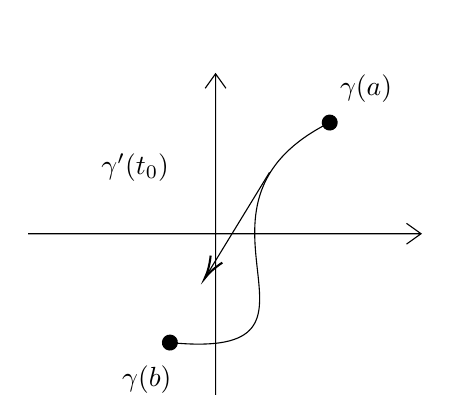
\begin{tikzpicture}[x=0.75pt,y=0.75pt,yscale=-1,xscale=1]
        %uncomment if require: \path (0,286); %set diagram left start at 0, and has height of 286
        
        %Shape: Axis 2D [id:dp5992461788507699] 
        \draw  (50,141.08) -- (239.26,141.08)(140.26,64) -- (140.26,226.51) (232.26,136.08) -- (239.26,141.08) -- (232.26,146.08) (135.26,71) -- (140.26,64) -- (145.26,71)  ;
        %Curve Lines [id:da8169369769076535] 
        \draw    (118.26,193.51) .. controls (210.26,202.51) and (113.26,128.51) .. (195.26,87.51) ;
        \draw [shift={(195.26,87.51)}, rotate = 333.43] [color={rgb, 255:red, 0; green, 0; blue, 0 }  ][fill={rgb, 255:red, 0; green, 0; blue, 0 }  ][line width=0.75]      (0, 0) circle [x radius= 3.35, y radius= 3.35]   ;
        \draw [shift={(118.26,193.51)}, rotate = 5.59] [color={rgb, 255:red, 0; green, 0; blue, 0 }  ][fill={rgb, 255:red, 0; green, 0; blue, 0 }  ][line width=0.75]      (0, 0) circle [x radius= 3.35, y radius= 3.35]   ;
        %Straight Lines [id:da7279313778056917] 
        \draw    (166.26,111.51) -- (136.05,160.92) ;
        \draw [shift={(135,162.63)}, rotate = 301.44] [color={rgb, 255:red, 0; green, 0; blue, 0 }  ][line width=0.75]    (10.93,-3.29) .. controls (6.95,-1.4) and (3.31,-0.3) .. (0,0) .. controls (3.31,0.3) and (6.95,1.4) .. (10.93,3.29)   ;
        
        % Text Node
        \draw (199,63.4) node [anchor=north west][inner sep=0.75pt]    {$\gamma ( a)$};
        % Text Node
        \draw (94,203.4) node [anchor=north west][inner sep=0.75pt]    {$\gamma ( b)$};
        % Text Node
        \draw (84,101.4) node [anchor=north west][inner sep=0.75pt]    {$\gamma '( t_{0})$};
        
        
        \end{tikzpicture}
\]

\defn Parameterize $\gamma(t)=(x(t), y(t))=x(t)+iy(t)$. Then $\gamma'(t_0)=(x'(t_0), y'(t_0))$ is a \textbf{tangent vector} to the curve at $\gamma(t_0)$ (assume $\gamma'(t_0)\neq \mathbf{0}$, aka. $\gamma$ is regular at $\gamma(t_0)$.)

\begin{theorem}[The ``Boxy-path'' Theorem]
    A nonempty open set $\Omega$ in $\C$ is connected \textit{if and only if} each pair of distinct
points in $\Omega$ can be joined by a sequence of line segments lying in $\Omega$, each of which is
parallel to either to the real or imaginary axis.
    \drawing{0.6\linewidth}{image-3.png}
    In other words, between any 2 points in a region $\reg$ there exists a ``\textbf{boxy path}''.
\end{theorem}

\rmk There is also always a \textbf{smooth path}. That is: \drawing{150pt}{image-4.png}

\begin{theorem}[``Smooth-path'']
    A nonempty open set $\reg$ in $\C$ is connected if and only if each pair of distinct
points in $\reg$ can be joined by a continuously differentiable curve in $\reg$ that is regular at
every point.
\end{theorem}
\begin{proof}
    See \href{https://stephangarcia.sites.pomona.edu/teaching/24S-135/Lecture/24S-135-Lecture02.pdf}{lecture 2 notes}.
\end{proof}

\subsection{Conformality}
Let $f$ be an analytic complex function on $\reg$.

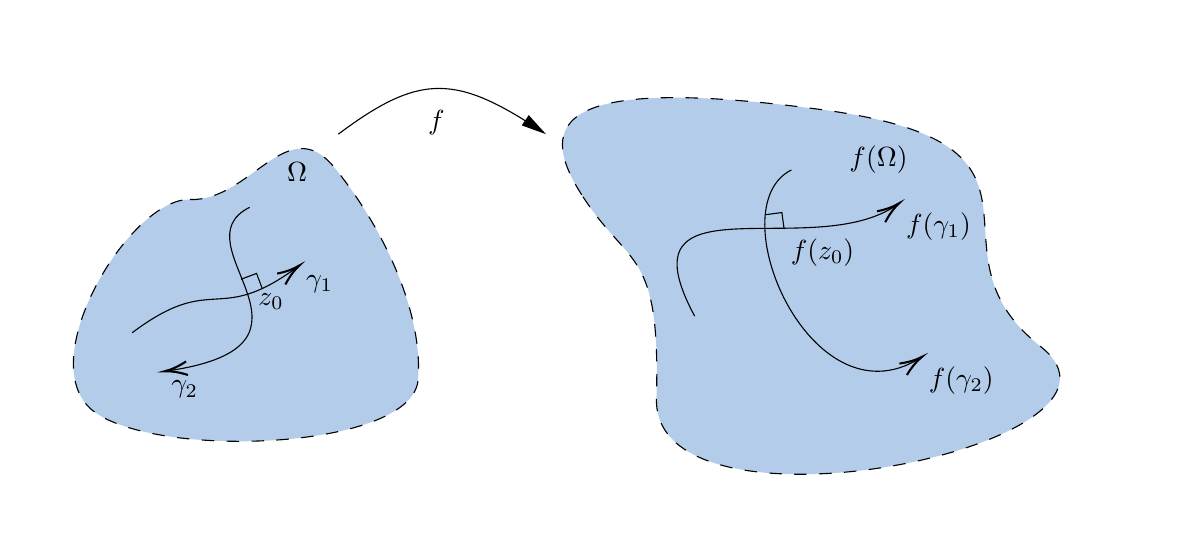
\begin{tikzpicture}[x=0.75pt,y=0.75pt,yscale=-1,xscale=1]
    %uncomment if require: \path (0,300); %set diagram left start at 0, and has height of 300
    
    %Shape: Polygon Curved [id:ds04152892949921583] 
    \draw  [fill={rgb, 255:red, 0; green, 87; blue, 184 }  ,fill opacity=0.3 ][dash pattern={on 4.5pt off 4.5pt}] (92.5,102.5) .. controls (121.5,103.5) and (139.5,59.5) .. (162,87) .. controls (184.5,114.5) and (204.91,155.75) .. (202.42,189.25) .. controls (199.92,222.75) and (79.59,227.75) .. (47.08,205.25) .. controls (14.58,182.75) and (63.5,101.5) .. (92.5,102.5) -- cycle ;
    %Curve Lines [id:da38490573070321243] 
    \draw    (64.67,166.67) .. controls (104.27,136.97) and (105.24,163.7) .. (144.07,135.13) ;
    \draw [shift={(145.25,134.25)}, rotate = 143.13] [color={rgb, 255:red, 0; green, 0; blue, 0 }  ][line width=0.75]    (10.93,-3.29) .. controls (6.95,-1.4) and (3.31,-0.3) .. (0,0) .. controls (3.31,0.3) and (6.95,1.4) .. (10.93,3.29)   ;
    %Curve Lines [id:da9683797356751562] 
    \draw    (121.25,106.25) .. controls (85.43,124.16) and (167.43,172.76) .. (81.56,185.07) ;
    \draw [shift={(80.25,185.25)}, rotate = 352.23] [color={rgb, 255:red, 0; green, 0; blue, 0 }  ][line width=0.75]    (10.93,-3.29) .. controls (6.95,-1.4) and (3.31,-0.3) .. (0,0) .. controls (3.31,0.3) and (6.95,1.4) .. (10.93,3.29)   ;
    %Shape: Right Angle [id:dp0014762610750393979] 
    \draw   (117.1,140.91) -- (124.59,138.1) -- (127.4,145.59) ;
    %Shape: Polygon Curved [id:ds020760136591730705] 
    \draw  [fill={rgb, 255:red, 0; green, 87; blue, 184 }  ,fill opacity=0.3 ][dash pattern={on 4.5pt off 4.5pt}] (281.25,100.25) .. controls (258.25,64.25) and (271.25,42.25) .. (397.25,59.25) .. controls (523.25,76.25) and (442.25,126.25) .. (502.25,173.25) .. controls (562.25,220.25) and (315.25,271.25) .. (317.25,198.25) .. controls (319.25,125.25) and (304.25,136.25) .. (281.25,100.25) -- cycle ;
    %Curve Lines [id:da5067199553805877] 
    \draw    (335.67,158.67) .. controls (298.63,89.94) and (392.35,133.36) .. (433.04,105.13) ;
    \draw [shift={(434.25,104.25)}, rotate = 143.13] [color={rgb, 255:red, 0; green, 0; blue, 0 }  ][line width=0.75]    (10.93,-3.29) .. controls (6.95,-1.4) and (3.31,-0.3) .. (0,0) .. controls (3.31,0.3) and (6.95,1.4) .. (10.93,3.29)   ;
    %Curve Lines [id:da12902529814050778] 
    \draw    (382.25,88.25) .. controls (346.61,106.07) and (391.34,211.12) .. (443.67,179.26) ;
    \draw [shift={(445.25,178.25)}, rotate = 146.56] [color={rgb, 255:red, 0; green, 0; blue, 0 }  ][line width=0.75]    (10.93,-3.29) .. controls (6.95,-1.4) and (3.31,-0.3) .. (0,0) .. controls (3.31,0.3) and (6.95,1.4) .. (10.93,3.29)   ;
    %Shape: Right Angle [id:dp16473621622546486] 
    \draw   (369.76,109.81) -- (377.69,108.76) -- (378.75,116.69) ;
    %Curve Lines [id:da7241992906101147] 
    \draw    (164,71) .. controls (203.6,41.3) and (220.91,42.23) .. (262.73,70.15) ;
    \draw [shift={(264,71)}, rotate = 213.92] [fill={rgb, 255:red, 0; green, 0; blue, 0 }  ][line width=0.08]  [draw opacity=0] (12,-3) -- (0,0) -- (12,3) -- cycle    ;
    
    % Text Node
    \draw (138,83.4) node [anchor=north west][inner sep=0.75pt]    {$\Omega $};
    % Text Node
    \draw (147.25,137.65) node [anchor=north west][inner sep=0.75pt]    {$\gamma _{1}$};
    % Text Node
    \draw (82.25,188.65) node [anchor=north west][inner sep=0.75pt]    {$\gamma _{2}$};
    % Text Node
    \draw (124.25,146.65) node [anchor=north west][inner sep=0.75pt]    {$z_{0}$};
    % Text Node
    \draw (409,75.4) node [anchor=north west][inner sep=0.75pt]    {$f( \Omega )$};
    % Text Node
    \draw (436.25,107.65) node [anchor=north west][inner sep=0.75pt]    {$f( \gamma _{1})$};
    % Text Node
    \draw (447.25,181.65) node [anchor=north west][inner sep=0.75pt]    {$f( \gamma _{2})$};
    % Text Node
    \draw (380.75,120.09) node [anchor=north west][inner sep=0.75pt]    {$f( z_{0})$};
    % Text Node
    \draw (206,58.4) node [anchor=north west][inner sep=0.75pt]    {$f$};
    
    
\end{tikzpicture}

Let $z_0\in \reg$ such that $f'(z_0)\neq 0$. Let $\gamma_1, \gamma_2$ be two curves that pass through $z_0$ intersecting with an angle $\theta$. Then $f(\gamma_1), f(\gamma_2)$ are two curves in $f(\Omega)$ passing through $f(\zeta_0)$ also with angle $\theta$.

Therefore, $f$ is \textbf{conformal}!

\section{Cauchy-Riemann equations, harmonic functions}
\subsection{Multivariate notion of complex derivatives}
Recall: $\displaystyle f'(z_0)=\lim_{h\to 0}\frac{f(z_0+h)-f(z_0)}{h}$.

Now we write each function with complex variables as $f(z)=u(z)+i\, v(z)$ where $u,v$ are real-valued \sidenote{meaning their range is real} functions.

Since $\C\cong \R^2$, we denote every point $z=(x,y)$.

Now we let $f(x,y)=u(x,y)+i\,v(x,y)$. We first let the small distance $h=(r,0)$ be horizontally approaching 0 with $r\in \R$. That is, $z_0+h=(x_0+r,y_0)$.
\begin{align*}
    f'(z_0) &= \lim_{r\to 0} \frac{u(x_0+r, y_0)-u(x_0,y_0)}{r} + i\cdot \lim_{r\to 0}\frac{v(x_0+r, y_0)-v(x_0,y_0)}{r}\\
    &=u_x(x_0,y_0)+i\cdot v_x(x_0,y_0)
\end{align*}

Similarly, if we vertically let $h=ir=(0,r)$ with $r\to 0, r\in \R$, we would get $f'=v_y-i\cdot u_y$.

\rmk If a derivative exists, the horizontal \& the vertical ones should be equal!

\begin{theorem}[Cauchy-Riemann Equations]
    \begin{align*}
        u_x &=v_y\\
        u_y &= -v_x
    \end{align*}
\end{theorem}\addlink{Cauchy-Riemann Equations}

\begin{corollary}
    If $f:\reg \to \C$ is analytic and $f'=0$ on $\reg$, then $f$ is \textbf{constant}.
\end{corollary}
\begin{proof}
    Since $0=f'=u_x+iv_x$, we see that $u_x=v_x=0$ on $\reg$. By Cauchy-Riemann, $v_y=u_y=0$ is also true on $\reg$. Hence, $\mathbf{u}, \mathbf{v}$ are constant on either horizontal or vertical segments. By the Boxy Path Theorem, $f=u+iv$ cannot assume two distinct values in $\reg$.
\end{proof}

\subsection{Orientation-preserving as shown by Jacobian}
Let $f:\reg \to \C$ be analytic. Then $f'=u_x+iv_x$ and hence:\begin{align*}
    |f'|^2 = \bar f'\cdot f &= (u_x-iv_x)(u_x+iv_x)\\
    &= u_x^2 + v_x^2\\
    &= u_xu_x+v_xv_x && \text{and by Cauchy-Riemann,}\\
    &= u_xv_y-u_yv_x\\
    &= \det\left(\begin{bmatrix}
        u_x & u_y\\
        v_x & v_y
    \end{bmatrix}\right) && \text{the Jacobian of $f$!}
\end{align*}

Since $|f'|^2\geq 0$, the determinant of the Jacobian is always $\geq 0$, implying that $f$ is always locally orientation-preserving. Moreover,

\begin{proposition}
    If $f'(z_0)\neq 0$, then $|f'|^2> 0$ implies:
    \begin{enumerate}
        \item $f$ is \textbf{injective} near $z_0$
        \item $f$ scales $\R$ by $|f'(z_0)|^2$ near $z_0$
        \item $f$ preserves orientation near $z_0$
    \end{enumerate}
\end{proposition}

\subsection{The Laplacian, harmonic functions and conjugates}
Suppose that $f=u+iv$ is analytic and $u,v$ have continuous second partial derivatives. Then:\begin{align*}
    u_{xx}+u_{yy} = \Delta u = (v_y)_x + (-v_x)_y = v_{yx}-v_{xy}=0
\end{align*}
This means that the Laplacian of this function $u$ is 0!\sidenote{$\Delta u = 0$ characterizes steady-state solutions to heat equations on $\reg$.}

\defn Real-valued functions $u: \reg\to \R$ satisfying that the Laplacian $\Delta u= u_{xx}+u_{yy}$ is 0 on $\reg$ is called \textbf{harmonic functions}.

\defn A \textbf{harmonic conjugate} of $u$ is a harmonic function $v: \reg \to \R$ such that $f=u+i\cdot v$ is \textbf{analytic} on $\reg$.
\addlink{Harmonic conjugate}

\eg $u=x^2-y^2, v=2xy$.\sidenote{Check it!}

\rmk Harmonic conjugates are unique up to translation (± constants).

\rmk If $u$ is harmonic on $\reg$, it does NOT have to have a harmonic conjugate on $\reg$.

\subsection{Finding a harmonic conjugate}
Recall that the real and imaginary parts of an analytic function are \textbf{harmonic}, in addition to satisfying the Cauchy-Riemann Equations: $u_x=v_y$ and $u_y=-v_x$.

\eg $u(z)=\log |z|$ is harmonic on $\C\backslash\{0\}$.
\begin{proof}
    Write $u(x,y)=\log (\sqrt{x^2+y^2})=\frac{1}{2}\log(x^2+y^2)$.

    Then, \begin{align*}
        u_x&=\frac{\partial}{\partial x}\left(\frac{1}{2}\log (x^2+y^2)\right)\\
        &= \frac{1}{2}\cdot \frac{2x}{x^2+y^2}\\
        &= \frac{x}{x^2+y^2}
    \end{align*}

    Hence,\sidenote{Review quotient rule!}
    \begin{align*}
        u_{xx} &= \frac{(x^2+y^2)-x(2x)}{(x^2+y^2)^2}\\
        &= \frac{y^2-x^2}{(x^2+y^2)^2}
    \end{align*}

    Symmetrically, we find \begin{align*}
        u_{yy} & = \frac{x^2-y^2}{(x^2+y^2)^2}
    \end{align*}
    Hence $u_{xx}+u_{yy}=0$, implying that the function is harmonic.
\end{proof}

Now, can we \uline{find a harmonic conjugate for the aforementioned $u$}?\sidenote{There is currently a great \textbf{CAVEAT} in all of these, because $v(z)=\arg(z)$ cannot be defined in a continuous manner in all of $\C\backslash\{0\}$: 

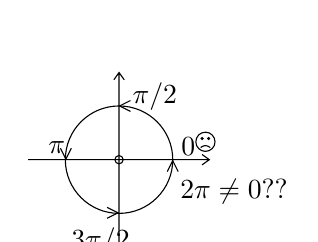
\begin{tikzpicture}[x=0.75pt,y=0.75pt,yscale=-0.5,xscale=0.5]
    %uncomment if require: \path (0,300); %set diagram left start at 0, and has height of 300
    
    %Shape: Axis 2D [id:dp48156480156165227] 
    \draw  (111,139) -- (285.5,139)(198.5,55) -- (198.5,219) (278.5,134) -- (285.5,139) -- (278.5,144) (193.5,62) -- (198.5,55) -- (203.5,62)  ;
    %Shape: Circle [id:dp6012967995903811] 
    \draw   (146.75,139) .. controls (146.75,110.42) and (169.92,87.25) .. (198.5,87.25) .. controls (227.09,87.25) and (250.26,110.42) .. (250.26,139) .. controls (250.26,167.58) and (227.09,190.75) .. (198.5,190.75) .. controls (169.92,190.75) and (146.75,167.58) .. (146.75,139) -- cycle ;
    \draw   (209.5,92.5) -- (199,87.25) -- (209.5,82) ;
    \draw   (152.5,128) -- (147.25,138.5) -- (142,128) ;
    \draw   (187,185) -- (197.5,190.25) -- (187,195.5) ;
    \draw   (245,150.5) -- (250.25,140) -- (255.5,150.5) ;
    %Shape: Smiley Face [id:dp013237994815757492] 
    \draw   (272.5,121.75) .. controls (272.5,116.64) and (276.64,112.5) .. (281.75,112.5) .. controls (286.86,112.5) and (291,116.64) .. (291,121.75) .. controls (291,126.86) and (286.86,131) .. (281.75,131) .. controls (276.64,131) and (272.5,126.86) .. (272.5,121.75) -- cycle ; \draw   (277.68,118.61) .. controls (277.68,118.09) and (278.09,117.68) .. (278.61,117.68) .. controls (279.12,117.68) and (279.53,118.09) .. (279.53,118.61) .. controls (279.53,119.12) and (279.12,119.53) .. (278.61,119.53) .. controls (278.09,119.53) and (277.68,119.12) .. (277.68,118.61) -- cycle ; \draw   (283.97,118.61) .. controls (283.97,118.09) and (284.38,117.68) .. (284.9,117.68) .. controls (285.41,117.68) and (285.82,118.09) .. (285.82,118.61) .. controls (285.82,119.12) and (285.41,119.53) .. (284.9,119.53) .. controls (284.38,119.53) and (283.97,119.12) .. (283.97,118.61) -- cycle ; \draw   (277.13,127.3) .. controls (280.21,124.83) and (283.29,124.83) .. (286.38,127.3) ;
    %Shape: Circle [id:dp5943162664556252] 
    \draw   (194.51,139) .. controls (194.51,136.79) and (196.3,135) .. (198.5,135) .. controls (200.71,135) and (202.5,136.79) .. (202.5,139) .. controls (202.5,141.21) and (200.71,143) .. (198.5,143) .. controls (196.3,143) and (194.51,141.21) .. (194.51,139) -- cycle ;
    
    % Text Node
    \draw (256,115.4) node [anchor=north west][inner sep=0.75pt]    {$0$};
    % Text Node
    \draw (209,62.4) node [anchor=north west][inner sep=0.75pt]    {$\pi /2$};
    % Text Node
    \draw (128,119.4) node [anchor=north west][inner sep=0.75pt]    {$\pi $};
    % Text Node
    \draw (150,202.4) node [anchor=north west][inner sep=0.75pt]    {$3\pi /2$};
    % Text Node
    \draw (255,155.4) node [anchor=north west][inner sep=0.75pt]    {$2\pi \neq 0??$};
    
    
    \end{tikzpicture}
    

To be resolved later!}

We could use the two Cauchy-Riemann Equations. One of them:
\begin{align*}
    v_y&=u_x\\
    &= \frac{x}{x^2+y^2}
\end{align*}
Therefore, \begin{align*}
    v(x,y) &= \int v_ydy + C(x) && \text{unknown function of }x\\
    &= \arctan\left(\frac{y}{x}\right)+C(x)
\end{align*}

Then, we use the second one: \begin{align*}
    \frac{y}{x^2+y^2}=u_y=-v_x &= -\frac{\partial}{\partial x} \left( \arctan\left(\frac{y}{x}\right)+C(x)\right)\\
    &= \frac{y}{x^2+y^2}-C'(x) \implies C'(x)=0
\end{align*}

Hence, a good harmonic conjugate candidate seems to be \begin{align*}
    v(x,y) = \arctan\left(\frac{y}{x}\right) + C
\end{align*}
where $C$ is a constant. WLOG, let $C=0$. Then $ v(x,y)=\arctan\left(\frac{y}{x}\right)$, meaning that: \begin{align*}
    v(z)=\arg (z)
\end{align*}

Therefore, $f(z)=\log |z| + i\cdot \arg(z)$ is analytic!
%%%%%%%

\subsection{Physics analogies of harmonic functions}
\eg Let $T(x,y,t)$ be the temperature at $(x,y)$ at time $t$ of a thermally conductive plate in $\C$. Assume the plate gives rise to a \textbf{bounded} region $\Omega$ (with boundary denoted $\partial \Omega$). Temperature on $\partial \Omega$ is a fixed function (time-independent).

\begin{figure}[H]
    \centering
    
\includegraphics[width=80pt]{Images/image-2.png}
\end{figure}

Now given the heat equation: \begin{align*}
    \frac{\partial T}{\partial t}-\alpha \Delta T=0
\end{align*}
where $\alpha$ is a constant.

We think the system tends towards a thermal equilibrium as $t\to \infty$. At equilibrium, $\frac{\partial T}{\partial t}$ is \textbf{zero}. Hence, at equilibrium, $\Delta T=T_{xx}+T_{yy}=0$.

\textbf{\underline{Idea}}: Harmonic function behave like equilibrium temperature distributions!

\begin{proposition}
    Let $U(x,y)$ be a harmonic function on $\Omega$.
    \begin{enumerate}
        \item $U$ cannot have a \textit{local} maximum in $\Omega$.
        \item The absolute maximum of $U$ on $\Omega ^-$\sidenote{$\Omega ^-$ denotes the closure of $\Omega$} occurs on $\partial \Omega$.
        \item $U$ cannot be locally constant without being globally constant.
    \end{enumerate}
\end{proposition}

\begin{theorem}[Maximum principle]
    Let $\Omega$ be a bounded region in $\C$ and let $f: \Omega^-\to \C$ be analytic on $\Omega$ and continuous on $\Omega^-$.
    \begin{enumerate}
        \item If $|f|$ achieves a local max in $\Omega$, then $f$ is constant.
        \item The global max of $|f|$ on $\Omega^-$ is attained on $\partial \Omega$.
    \end{enumerate}
\end{theorem}

\section{Möbius transformations}
\subsection{Möbius transformations, the extended plane}
\defn[Möbius transformations]
\begin{align*}
    f(z)=\frac{az+b}{cz+d}\text{ where } ad-bc\neq 0, a,b,c,d\in \C
\end{align*}
Such an $f$ is \textbf{analytic} on $\C\backslash\{\frac{-d}{c}\}$\sidenote{recall that rational functions are analytic except when the denominator vanishes, i.e. $cz+d\neq 0$.} and \textbf{comformal} there since $f'(z)=\frac{ad-bc}{(cz+d)^2}\neq 0$ on $\C\backslash\{\frac{-d}{c}\}$.

\rmk In addition, $f$ is injective (one-to-one)!
\begin{proof}
    \begin{align*}
        f(z)=f(w)\implies \frac{az+b}{cz+d}&=\frac{aw+b}{cw+d}\\
         (az+b)(cw+d)&= (cz+d)(aw+b)\\
         aczw+bcw+adz+bd&=aczw+adw+bcz+bd\\
         (ad-bc)z&=(ad-bc)w\\
         z&=w
    \end{align*}
\end{proof}

\defn[The extended plane] We set the following convention:\begin{align*}
    f(\frac{-d}{c})&= \infty\\
    f(\infty) &= \frac{a}{c}
\end{align*}
with this, $f$ is a \textbf{bijection} from $\Chat=\C\cup\{\infty\}$ to itself.\sidenote{recall Riemann sphere}

\subsection{Möbius transformations as matrices}
\rmk We can \textit{associate}\sidenote{this association is not a bijection: it's only so up to scaling} $f(z)=\frac{az+b}{cz+d}$ where $ad-bc\neq 0$ with the matrix $$M_f=\begin{bmatrix}
    a&b\\c&d
\end{bmatrix}$$

\rmk $M_{f\circ g}=M_f\cdot M_g$\sidenote{check this!}

\rmk The inverse of $M_f=\begin{bmatrix}
    a&b\\c&d
\end{bmatrix}$ is $M_f^{-1}=\frac{1}{ad-bc}\begin{bmatrix}
    d&-b\\-c&a
\end{bmatrix}$ and scaling does not matter, so we could write the \textbf{inverse} of such Möbius transformation as: \begin{align*}
    \inv{f}(w) &=\frac{dw-b}{-cw+a}
\end{align*}

\begin{theorem}
    A Möbius transformation $f:\Chat\to\Chat$ with three fixed points in $\Chat$ is the \textbf{identity map} $\mathrm{id}(z)=z=\frac{z+0}{0z+1}$.\sidenote{$I=\begin{bmatrix}
        1&0\\0&1
    \end{bmatrix}$}
\end{theorem}
\begin{proof}
    Let $f(z)=\frac{az+b}{cz+d}$ be a Möbius transformation.
    \begin{enumerate}
        \item If $\infty$ is fixed, then $c=0$\sidenote{think about that!}. Then $f(z)=\frac{a}{d}z+\frac{b}{d}$, which is a \textbf{linear} transformation.\begin{enumerate}
            \item If $f(z)=z$, we are done since we get the identity!
            \item Otherwise the function only has one fixed point at $\infty$.
        \end{enumerate}
        \item If $\infty$ is not a fixed point, then $c\neq 0$. Solve:\begin{align*}
            f(z)+z \Leftrightarrow \frac{az+b}{cz+d}&=z\\
            az+b&=cz^2+dz\\
            cz^2+(d-a)z-b&=0
        \end{align*}
        is a quadratic which has at most two (distinct) solutions in $\C$. Hence, this transformation fixes at most two points.
    \end{enumerate}
\end{proof}

\subsection{Möbius transformations take circles to circles}
\rmk Lines can be circles (they are just circles that pass through the point at infinity).

\begin{theorem}
    The image of a circle under a Möbius transformation is still a circle.
\end{theorem}
\begin{proof}
    Let $f(z)=\frac{az+b}{cz+d}$ be a Möbius transformation.
    \begin{enumerate}
        \item If $c=0$, then $f(z)=\frac{a}{d}z+\frac{b}{d}$, which is a \textbf{linear/affine} transformation and so we are done\sidenote{since linear transformations preserve circles and lines}.
        \item Now suppose $c\neq 0$. Then \begin{align*}
            f(z)&=\frac{a}{d}z+\frac{b}{d}\\
            &= \frac{\frac{a}{c}(cz+d)-\frac{ad}{c}+b}{cz+d}\\
            &= \frac{b-\frac{ad}{c}}{cz+d}+\frac{a}{c}
        \end{align*}
        which is a composition of affine, inversion and affine:
        $$z\mapsto cz+d\mapsto \frac{1}{cz+d}\mapsto \frac{b-\frac{ad}{c}}{cz+d}+\frac{a}{c}$$
        We now only need to show that inversion preserves circles.

        Let a circle in $\R^2$ be $Ax+By+C(x^2+y^2)=D$ where $A,B,C,D\in \R$. If $z=x+iy\in \Chat$, then $\frac{1}{z}=\frac{x}{x^2+y^2}+i\frac{-y}{x^2+y^2}$. Name $\frac{1}{z}=u+iv$, note that $u^2+v^2=\frac{1}{x^2+y^2}$. 
        
        Then we note that $Au-Bv+C=D(u^2+v^2)$\sidenote{check this!}, which is still a circle!
    \end{enumerate}
\end{proof}

\begin{theorem}
    Given two triples $z_1,z_2,z_3$ and $w_1,w_2,w_3$ of \textit{distinct} points in $\Chat$, then there is always a unique Möbius transformation $f$ such that $f(z_i)=w_i$ for all $i=1,2,3$.
\end{theorem}
\begin{proof}
    Claim: the \textit{cross-ratio} $\phi(z)=\frac{z-z_1}{z-z_3}\cdot \underset{\text{const.}}{\underbrace{\frac{z_2-z_3}{z_2-z_1}}}$ is a Möbius transformation that satisfies \circled{$\phi(z_1)=0, \phi(z_2)=1, \phi(z_3)=\infty$}.

    We can also find another Möbius transformation such that $\psi(z_1)=0, \psi(z_2)=1, \psi(z_3)=\infty$. Then:
    \[\begin{tikzcd}[ampersand replacement=\&,cramped,row sep=tiny]
        {z_1} \& 0 \& {w_1} \\
        {z_2} \& 1 \& {w_2} \\
        {z_3} \& \infty \& {w_3}
        \arrow["\phi", maps to, from=1-1, to=1-2]
        \arrow["{\psi^{-1}}", maps to, from=1-2, to=1-3]
        \arrow["\phi", maps to, from=2-1, to=2-2]
        \arrow["{\psi^{-1}}", maps to, from=2-2, to=2-3]
        \arrow["\phi", maps to, from=3-1, to=3-2]
        \arrow["{\psi^{-1}}", maps to, from=3-2, to=3-3]
    \end{tikzcd}\]

    and we could simply let $f=\psi^{-1}\circ \phi$.
\end{proof}

\eg Let $f(z)=\frac{z+1}{-z+1}$. We compute:\begin{align*}
    f(0)&=1\\
    f(-1)&=0\\
    f(1)&=\infty\\
    f(i)&=i\\
    f(-i)&=-i\\
\end{align*}

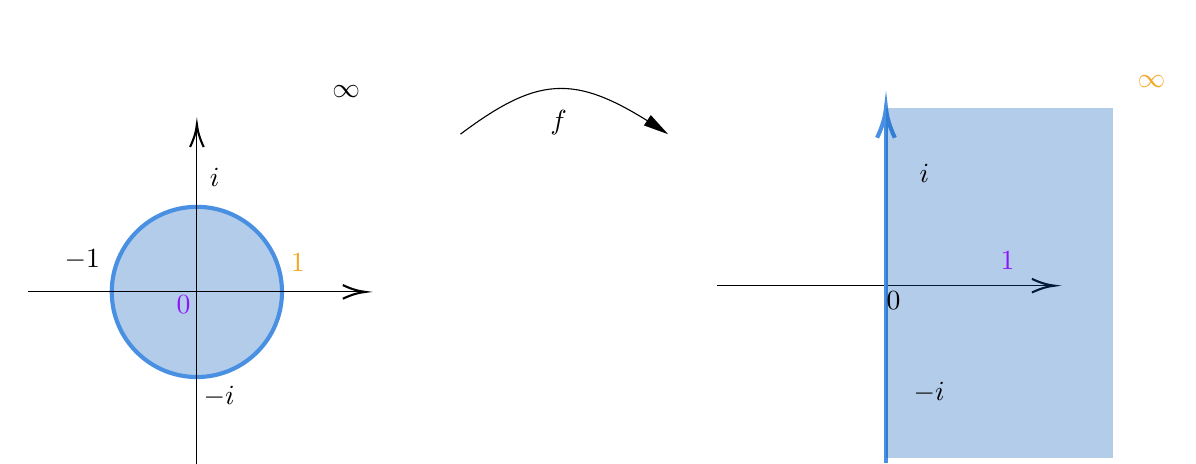
\begin{tikzpicture}[x=0.75pt,y=0.75pt,yscale=-1,xscale=1]
%uncomment if require: \path (0,300); %set diagram left start at 0, and has height of 300

%Shape: Circle [id:dp46487660565461075] 
\draw  [color={rgb, 255:red, 74; green, 144; blue, 226 }  ,draw opacity=1 ][fill={rgb, 255:red, 0; green, 87; blue, 184 }  ,fill opacity=0.3 ][line width=1.5]  (96,156.01) .. controls (96,133.37) and (114.36,115.01) .. (137.01,115.01) .. controls (159.65,115.01) and (178.01,133.37) .. (178.01,156.01) .. controls (178.01,178.66) and (159.65,197.02) .. (137.01,197.02) .. controls (114.36,197.02) and (96,178.66) .. (96,156.01) -- cycle ;
%Curve Lines [id:da6037660096213038] 
\draw    (264,80) .. controls (303.6,50.3) and (320.91,51.23) .. (362.73,79.15) ;
\draw [shift={(364,80)}, rotate = 213.92] [fill={rgb, 255:red, 0; green, 0; blue, 0 }  ][line width=0.08]  [draw opacity=0] (12,-3) -- (0,0) -- (12,3) -- cycle    ;
%Straight Lines [id:da30485423184171] 
\draw    (55.75,156.01) -- (216.26,156.01) ;
\draw [shift={(218.26,156.01)}, rotate = 180] [color={rgb, 255:red, 0; green, 0; blue, 0 }  ][line width=0.75]    (10.93,-3.29) .. controls (6.95,-1.4) and (3.31,-0.3) .. (0,0) .. controls (3.31,0.3) and (6.95,1.4) .. (10.93,3.29)   ;
%Straight Lines [id:da03496103337291223] 
\draw    (387.75,153.01) -- (548.26,153.01) ;
\draw [shift={(550.26,153.01)}, rotate = 180] [color={rgb, 255:red, 0; green, 0; blue, 0 }  ][line width=0.75]    (10.93,-3.29) .. controls (6.95,-1.4) and (3.31,-0.3) .. (0,0) .. controls (3.31,0.3) and (6.95,1.4) .. (10.93,3.29)   ;
%Straight Lines [id:da11880027193931353] 
\draw    (137.01,246.26) -- (137.01,77.26) ;
\draw [shift={(137.01,75.26)}, rotate = 90] [color={rgb, 255:red, 0; green, 0; blue, 0 }  ][line width=0.75]    (10.93,-3.29) .. controls (6.95,-1.4) and (3.31,-0.3) .. (0,0) .. controls (3.31,0.3) and (6.95,1.4) .. (10.93,3.29)   ;
%Straight Lines [id:da4256972022746721] 
\draw [color={rgb, 255:red, 74; green, 144; blue, 226 }  ,draw opacity=1 ][line width=1.5]    (469.01,238.51) -- (469.01,70.51) ;
\draw [shift={(469.01,67.51)}, rotate = 90] [color={rgb, 255:red, 74; green, 144; blue, 226 }  ,draw opacity=1 ][line width=1.5]    (14.21,-4.28) .. controls (9.04,-1.82) and (4.3,-0.39) .. (0,0) .. controls (4.3,0.39) and (9.04,1.82) .. (14.21,4.28)   ;
%Shape: Rectangle [id:dp17327106892852906] 
\draw  [draw opacity=0][fill={rgb, 255:red, 0; green, 87; blue, 184 }  ,fill opacity=0.3 ] (469.01,67.51) -- (578.26,67.51) -- (578.26,236.26) -- (469.01,236.26) -- cycle ;

% Text Node
\draw (142,95.4) node [anchor=north west][inner sep=0.75pt]    {$i$};
% Text Node
\draw (181,136.4) node [anchor=north west][inner sep=0.75pt]  [color={rgb, 255:red, 245; green, 166; blue, 35 }  ,opacity=1 ]  {$1$};
% Text Node
\draw (139.01,200.42) node [anchor=north west][inner sep=0.75pt]    {$-i$};
% Text Node
\draw (72,134.4) node [anchor=north west][inner sep=0.75pt]    {$-1$};
% Text Node
\draw (126,156.4) node [anchor=north west][inner sep=0.75pt]  [color={rgb, 255:red, 144; green, 19; blue, 254 }  ,opacity=1 ]  {$0$};
% Text Node
\draw (484,93.4) node [anchor=north west][inner sep=0.75pt]    {$i$};
% Text Node
\draw (523,135.4) node [anchor=north west][inner sep=0.75pt]  [color={rgb, 255:red, 144; green, 19; blue, 254 }  ,opacity=1 ]  {$1$};
% Text Node
\draw (481.01,198.42) node [anchor=north west][inner sep=0.75pt]    {$-i$};
% Text Node
\draw (468,154.4) node [anchor=north west][inner sep=0.75pt]    {$0$};
% Text Node
\draw (201,55.4) node [anchor=north west][inner sep=0.75pt]    {$\infty $};
% Text Node
\draw (306,67.4) node [anchor=north west][inner sep=0.75pt]    {$f$};
% Text Node
\draw (589,50.4) node [anchor=north west][inner sep=0.75pt]    {$\textcolor[rgb]{0.96,0.65,0.14}{\infty }$};


\end{tikzpicture}

\section{Recall: infinite series}
\defn $\sum_{n=1}^{\infty}a_n$ converges to $S$ if $\lim_{N\to \infty}S_N=S$ where $S_N=a_1+\dots+a_N$.\sidenote{$S_N$ is the $N$-th partial sum.}

\subsection{Divergence test}
\defn[Divergence test]A pair of contrapositives:\sidenote{Note it's not an \ifnif !}\begin{enumerate}
    \item If $\sum_{n=1}^{\infty}a_n$ converges, then $\lim_{n\to\infty}a_n=0$.
    \item If $\lim_{n\to\infty}a_n\neq 0$ (\textit{including the case where the limit doesn't exist}) then $\sum_{n=1}^{\infty}a_n$ diverges.
\end{enumerate}
\noneg The harmonic series $\sum_{n=1}^{\infty}\frac{1}{n}=1+\frac{1}{2}+\dots$ diverges\sidenote{diverges, but really \textbf{slowly}!} even though $a_n=\frac{1}{n}$ tends to 0 when $n$ tends to $\infty$.

\begin{theorem}
    If $\sum_{n=1}^{\infty}a_n$ converges, then $\lim_{N\to \infty}\sum_{n=N}^{\infty}a_n=\lim_{N\to \infty}S-S_N=0$.\sidenote{In other words, the tail of a convergent series goes to 0.}
\end{theorem}

\begin{theorem}[Cauchy Criterion]
    $\sum_{n=1}^{\infty}a_n$ converges \ifnif for all $\varepsilon>0$, there exists $N\in \N$ such that $k>j>N$ implies $\displaystyle \left|\sum_{n=j-1}^{k}a_n \right|=S_k-S_j<\varepsilon$.
\end{theorem}

\subsection{Integral test}

\defn[Integral test] Define $a_n=f(n)$ for $n\in \N$, where $f:[1,\infty[ \to \R$ is (piecewise) continuous, positive and decreasing. Then $\int_{1}^{\infty}f(x)\, \d x$ converges \ifnif $\sum_{n=1}^{\infty}a_n$ converges.\sidenote{do an improper integral!}

Moreover, $\int_{1}^{N}f(x)\,\d x\leq a_1+\dots+a_N\leq a_1+\int_{1}^{N}f(x)\,\d x$.

\eg Apply the above with $f(x)=\frac{1}{x}$.\sidenote{$a_n=\frac{1}{n}$} Then \begin{align*}
    \ln N\leq 1+\frac{1}{2}+\dots+\frac{1}{N}\leq 1+\ln N
\end{align*}
It is bounded below by a divergent function, so it must be divergent!

\begin{theorem}
    The ``$p$-series'' $\sum_{n=1}^{\infty}\frac{1}{n^p}$ converges \ifnif $p>1$.
\end{theorem}

\defn[Riemann zeta function] \begin{align*}
    \zeta(s)&=\sum_{n=1}^{\infty}\frac{1}{n^s} && \text{for Re}(s)>1
\end{align*}
\rmk Euler figured out: \begin{align*}
    \zeta(2)&=\frac{\pi^2}{6}\\
    \zeta(4)&=\frac{\pi^4}{90}\\
    \zeta(6)&=\frac{\pi^6}{945}\\
    \vdots
\end{align*}
\rmk R. Apéry showed that $\zeta(3)$ is irrational (1979)\sidenote{still an open question in mathematics}:
\[\zeta(3)=\sum_{n=1}^{\infty}\frac{1}{n^3}=1.202\dots\]
but no explicit formula known!

\subsection{Absolute convergence}

\defn A series $\sum_{n=1}^{\infty}a_n$ is:\begin{enumerate}
    \item \textbf{absolutely convergent} if $\sum_{n=1}^{\infty}|a_n|$ converges.\sidenote{Good}
    \item \textbf{conditionally convergent} if $\sum_{n=1}^{\infty}a_n$ converges but $\sum_{n=1}^{\infty}|a_n|$ diverges.\sidenote{BAD}
\end{enumerate}

\begin{theorem}
    Every absolutely convergent series converges.
\end{theorem}
\eg The alternating harmonic series\sidenote{Don't re-parenthesize the terms -- grouping would change the sequence and thus the partial sums!} $$\sum_{n=1}^{\infty}\frac{(-1)^{n+1}}{n}=1-\frac{1}{2}+\frac{1}{3}-\frac{1}{4}+\dots$$ converges to $\ln 2$. But the convergence is conditional because the absolute value $$\sum_{n=1}^{\infty}\left|\frac{(-1)^{n+1}}{n}\right|=\sum_{n=1}^{\infty}\frac{1}{n}$$ does not converge.

\begin{theorem}
    An absolutely convergent series may be rearranged without changing its value. That is, if $\phi:\N\to \N$ is a bijection, then\sidenote{This seems obvious for finite series, but consider how this is extraordinary for infinite series!} $$\sum_{n=1}^{\infty}a_n=\sum_{n=1}^{\infty}a_{\phi(n)}$$
\end{theorem}

\addlink{Riemann Rearrangement Theorem}
\begin{theorem}[Riemann Rearrangement Theorem]
    If $\sum_{n=1}^{\infty}a_n$ is a \uline{conditionally convergent} series of real numbers, then for \textbf{any} $S\in \R\cup \{-\infty,\infty\}$, there is a bijection $\phi:\N\to\N$ such that $\sum_{n=1}^{\infty}a_{\phi(n)}=S$.\sidenote{Meaning we can get it to be equal to whatever we want just by rearranging!}
\end{theorem}

\spl

Now if $\sum_{n=0}^{\infty}a_n$ and $\sum_{n=0}^{\infty}b_n$ converge, one might expect that \begin{align*}
    \left(\sum_{i=0}^{\infty}a_i\right)\left(\sum_{j=0}^{\infty}b_j\right)&=(a_0+a_1+\dots)(b_0+b_1+\dots)\\
    &= a_0b_0+(a_0b_1+a_1b_0)+\dots\\
    &= \sum_{n=0}^{\infty}c_n \text{ where } c_n=\sum_{k=0}^{n}a_kb_{n-k}
\end{align*}
But this only works if both series are absolutely convergent, in which case the new series is absolutely convergent.\sidenote{conditionally convergent doesn't work! See \href{https://stephangarcia.sites.pomona.edu/teaching/24S-135/Lecture/24S-135-Lecture06.pdf}{notes}.}

\subsection{Uniform convergence}
\defn A sequence of functions $f_n: X\to \C$ where $X\subseteq \C$ \textbf{converges uniformly} to $f:X\to \C$ if for all $\varepsilon>0$, there exists a $N\in \N$ such that $n\geq N$ implies $|f_n(z)-f(z)|<\varepsilon$ for all $z\in X$.\sidenote{This is MATH131!}
\drawing{0.6\linewidth}{image-5.png}

\addlink{Uniform convergence preserves continuity}
\begin{theorem}
    If $f_n: X\to \C$ are continuous and converges uniformly on $X$ to $f:X\to\C$, then $f$ is continuous on $X$.\sidenote{unif. conv. preserves continuity}
    In other words, the uniform limit of continuous functions is continuous.
\end{theorem}

\rmk $f_n$ converges to $f$ pointwise on $X$ if $\lim_{n\to \infty}f_n(z)=f(z)$ for all $z\in X$.\sidenote{This doesn't say anything about the rate each point converges.}
\drawing{0.6\linewidth}{image-6.png}

\addlink{Integrals work with uniform convergence}
\begin{theorem}
    If $f_n:[a,b]\to \C$ are continuous and converge uniformly on $[a,b]$ to $f$, then\sidenote{Integrals work with uniform convergence} $$
    \lim_{n\to \infty}\int_{a}^{b}f_n(x)\,\d x = \int_{a}^{b}f(x)\,\d x
    $$
\end{theorem}

\rmk Uniform convergence doesn't necessarily preserve differentiability, limit or derivatives!

\eg $f_n(x)=\sqrt{x^2+\frac{1}{n}}$ on $[-1,1]$ converges uniformly to $f_n(x)=|x|$. But the limit function is \textbf{not} differentiable at $x=0$ even though every $f_n$ were.

\begin{theorem}[Weierstrass $M$-Test] 
    Let $f_n:X\to \C$ satisfy $|f_n(z)|\leq M_n$ for all $z\in X$ and $n\in \N$. If $\sum_{n=1}^{\infty}M_n$ converges, then $\sum_{n=1}^{\infty}f_n(z)$ converges both \textbf{absolutely} and \textbf{uniformly} on $X$.
\end{theorem}

\section{Power series}
\defn A \textbf{power series} is a series of the form $\sum_{n=0}^{\infty}a_n(z-z_0)^n$. The $a_n$ is the \textit{coefficient} and $z_0$ is the \textit{center}.

\subsection{Convergence of geometric series}

\begin{theorem}
    The \textit{geometric series} ($a_n=1, z_0=0$) $\sum_{n=0}^{\infty}z^n$ converges absolutely to $\frac{1}{1-z}$ if $|z|<1$, and it diverges otherwise. 

    Moreover, for each $r\in [0,1[$, the convergence is \textbf{uniform} on $|z|\leq r$.
\end{theorem}
\begin{proof}
    If $|z|\geq 1$, then $z^n\not\to 0$, so by the test of divergence, the series diverges.

    Now suppose $|z|<1$. Then\sidenote{The fact that we can find a formula for this sum is quite rare! } \begin{align*}
        \sum_{n=0}^{\infty}z^n &= \lim_{N\to \infty}\sum_{n=0}^{N-1}z^n\\
        &= \lim_{N\to \infty}(1+z+z^2+\dots+z^{N-1})\\
        &= \lim_{N\to \infty}\frac{1-z^N}{1-z}\\
        &= \frac{1}{1-z} &\text{since }|z|<1
    \end{align*}
    Which gives us point-wise convergence. Then, for any $r$ such that $|z|\leq r<1$, we have \begin{align*}
        \sum_{n=0}^{\infty}|z^n|\leq \sum_{n=0}^{\infty}r^n =\frac{1}{1-r}<\infty
    \end{align*}
    Hence, by the Weierstrass $M$-test, the series converges \textit{absolutely and uniformly} on $|z|\leq r$.
\end{proof}

\rmk Moral of the story: \begin{itemize}
    \item The \textit{radius of convergence} $R=1$ has the property that the series converges on $|z|<R$, and diverges if $|z|>R$.
    
    \item The series converges \textit{uniformly} on $|z|\leq r<1$ but not on $|z|<1$ itself. Why?
    
    Let $r=1$; we need be able to get $N\in \N$ such that for all $n\geq N$, we have $\left|\frac{1-z^N}{1-z}-\frac{1}{1-z}\right|<1$ for all $|z|<1$. However, this is not gonna work: as $z\to 1$, observe that this is going to eventually exceed 1. 

    \item The limit function $\displaystyle \frac{1}{1-z}$ is \textbf{analytic} on $\C\backslash\{1\}$\sidenote{the limit function is well-defined way beyond the $\mathbb{D}$!}. But the geometric series represents this function \underline{only} on $|z|<1$. In a smaller set, the power series represents the function that might originally be defined on a much larger set. The limit function is the \textit{analytic continuation} of the series.
    
    \item The limit function $\displaystyle \frac{1}{1-z}$ is cool if $z\neq 1$\sidenote{in the complex number sense!}, but as long as $|z|=1$ (\textbf{even} if $z\neq 1$), the geometric series diverges!
\end{itemize}

\subsection{Radius of convergence}
\defn The \textbf{limit superior} ($\limsup$) of a sequence of nonnegative real numbers $x_n$ is the largest \textit{limit point}\sidenote{limits of a subsequence of $x_n$} of the $x_n$: $$\limsup_{n\to \infty}x_n=\inf_{n\geq 0}\sup_{m\geq n}x_m$$\sidenote{the RHS as in real analysis}\addlink{Limit superior}
If the sequence is unbounded, the $\limsup$ would be $\infty$.

\eg If $x_n$ is the sequence $0,1,0,1,\dots$ then $\displaystyle\limsup_{n\to \infty}x_n=1$.

\eg If $x_n$ is the sequence $0,1,0,\frac{1}{2}, 0, \frac{1}{3},\dots$, then $\displaystyle\limsup_{n\to \infty}x_n=0$.

\rmk If $x_n$ are nonnegative, then \begin{itemize}
    \item $\displaystyle \limsup_{n\to \infty}(a_n+b_n)=\limsup_{n\to \infty}a_n+\limsup_{n\to \infty}b_n$
    \item $\displaystyle \limsup_{n\to \infty}(a_nb_n)\leq (\limsup_{n\to \infty}a_n)(\limsup_{n\to \infty}b_n)$
\end{itemize}

\addlink{Cauchy-Hadamard formula}
\begin{theorem}[Cauchy-Hadamard]
    Let $\sum_{n=0}^{\infty}a_n(z-z_0)^n$ be a power series. Define $R\in [0,\infty]$ by \sidenote{interpret $\frac{1}{0}=\infty$}\begin{align*}
        \frac{1}{R}=\limsup_{n\to \infty}\sqrt[n]{|a_n|}
    \end{align*}
    Then the $R$ is the \textit{radius of convergence}.
    \begin{enumerate}[label=(\alph*)]
        \item On $|z-z_0|<R$, the series converges \textbf{absolutely}.\sidenote{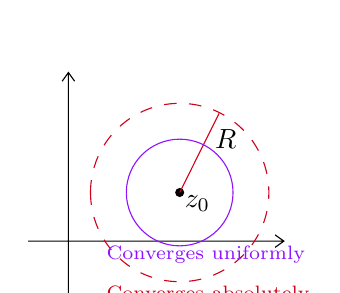
\begin{tikzpicture}[x=0.75pt,y=0.75pt,yscale=-0.6,xscale=.6]
            %uncomment if require: \path (0,300); %set diagram left start at 0, and has height of 300
            
            %Shape: Axis 2D [id:dp5858755410080565] 
            \draw  (50,212.68) -- (255.26,212.68)(82.26,77.28) -- (82.26,267.03) (248.26,207.68) -- (255.26,212.68) -- (248.26,217.68) (77.26,84.28) -- (82.26,77.28) -- (87.26,84.28)  ;
            %Shape: Circle [id:dp24544423482988642] 
            \draw  [color={rgb, 255:red, 208; green, 2; blue, 27 }  ,draw opacity=1 ][dash pattern={on 4.5pt off 4.5pt}] (100,173.64) .. controls (100,134.09) and (132.06,102.03) .. (171.61,102.03) .. controls (211.17,102.03) and (243.23,134.09) .. (243.23,173.64) .. controls (243.23,213.19) and (211.17,245.26) .. (171.61,245.26) .. controls (132.06,245.26) and (100,213.19) .. (100,173.64) -- cycle ;
            %Shape: Circle [id:dp09425242443966897] 
            \draw  [fill={rgb, 255:red, 0; green, 0; blue, 0 }  ,fill opacity=1 ] (168.46,173.64) .. controls (168.46,171.9) and (169.87,170.48) .. (171.61,170.48) .. controls (173.36,170.48) and (174.77,171.9) .. (174.77,173.64) .. controls (174.77,175.39) and (173.36,176.8) .. (171.61,176.8) .. controls (169.87,176.8) and (168.46,175.39) .. (168.46,173.64) -- cycle ;
            %Straight Lines [id:da3698233641764985] 
            \draw [color={rgb, 255:red, 208; green, 2; blue, 27 }  ,draw opacity=1 ]   (203.26,110.07) -- (171.61,173.64) ;
            %Shape: Circle [id:dp40259923856296376] 
            \draw  [color={rgb, 255:red, 144; green, 19; blue, 254 }  ,draw opacity=1 ] (128.79,173.64) .. controls (128.79,149.99) and (147.96,130.81) .. (171.61,130.81) .. controls (195.27,130.81) and (214.44,149.99) .. (214.44,173.64) .. controls (214.44,197.29) and (195.27,216.47) .. (171.61,216.47) .. controls (147.96,216.47) and (128.79,197.29) .. (128.79,173.64) -- cycle ;
            
            % Text Node
            \draw (198,120.82) node [anchor=north west][inner sep=0.75pt]    {$R$};
            % Text Node
            \draw (173.61,173.88) node [anchor=north west][inner sep=0.75pt]    {$z_{0}$};
            % Text Node
            \draw (110.8,246.42) node [anchor=north west][inner sep=0.75pt]  [color={rgb, 255:red, 208; green, 2; blue, 27 }  ,opacity=1 ] [align=left] {{\scriptsize Converges absolutely}};
            % Text Node
            \draw (110.8,214.62) node [anchor=north west][inner sep=0.75pt]   [align=left] {{\scriptsize \textcolor[rgb]{0.56,0.07,1}{Converges uniformly}}};
            
            
            \end{tikzpicture}} 
            For each $r\in [0,R[$, the convergence is \textbf{uniform} on $|z-z_0|\leq r$.        
        \item If $|z-z_0|>R$ then the series diverges. \rt{For $|z-z_0|=R$ anything could happen!}
    \end{enumerate}
\end{theorem}

\eg We claim that $\exp(z)=\sum_{n=0}^{\infty}\frac{z^n}{n!}$ has an infinite radius of convergence $R=\infty$. To check:
\begin{align*}
    \sqrt[n]{|a_n|} =\sqrt[n]{\frac{1}{n!}} = \frac{1}{\sqrt[n]{n!}}\to 0
\end{align*}
This is because $\sqrt[n]{n!} = \sqrt[n]{1\cdot 2\cdot\dots \cdot n}$, and in $n!$, there are at least $\frac{1}{2}$ terms that are $>\frac{n}{2}$. Thus, $\sqrt[n]{n!}\geq \left(\left(\frac{n}{2}\right)^{\frac{n}{2}}\right)^{\frac{1}{n}}=\left(\frac{n}{2}\right)^{1/2}\to \infty$.

So $R=\infty$ and we are done \begin{tikzpicture}[x=0.75pt,y=0.75pt,yscale=-.2,xscale=.2]%Shape: Smiley Face [id:dp9495597583093132] 
    \draw   (80,136) .. controls (80,116.67) and (95.67,101) .. (115,101) .. controls (134.33,101) and (150,116.67) .. (150,136) .. controls (150,155.33) and (134.33,171) .. (115,171) .. controls (95.67,171) and (80,155.33) .. (80,136) -- cycle ; \draw   (99.6,124.1) .. controls (99.6,122.17) and (101.17,120.6) .. (103.1,120.6) .. controls (105.03,120.6) and (106.6,122.17) .. (106.6,124.1) .. controls (106.6,126.03) and (105.03,127.6) .. (103.1,127.6) .. controls (101.17,127.6) and (99.6,126.03) .. (99.6,124.1) -- cycle ; \draw   (123.4,124.1) .. controls (123.4,122.17) and (124.97,120.6) .. (126.9,120.6) .. controls (128.83,120.6) and (130.4,122.17) .. (130.4,124.1) .. controls (130.4,126.03) and (128.83,127.6) .. (126.9,127.6) .. controls (124.97,127.6) and (123.4,126.03) .. (123.4,124.1) -- cycle ; \draw   (97.5,150) .. controls (109.17,159.33) and (120.83,159.33) .. (132.5,150) ;
    \end{tikzpicture}. We have that $\exp(z)$ has absolute convergence on the entire complex plane!

Absolute convergence means that we can multiply term-by-term:
\begin{align*}
    \exp(z)\exp(w) & = \left(\sum_{n=0}^{\infty}\frac{z^n}{n!}\right)\left(\sum_{n=0}^{\infty}\frac{w^n}{n!}\right)\\
    &= \sum_{n=0}^{\infty}\left(\sum_{k=0}^{\infty}\frac{z^k}{k!}\cdot\frac{w^{n-k}}{(n-k)!}\right)\\
    &= \sum_{n=0}^{\infty}\rt{\frac{1}{n!}}\underset{\text{binomial theorem}}{\underbrace{\sum_{k=0}^{\infty}\frac{\rt{n!}}{k!(n-k)!}z^kw^{n-k}}}\\
    &= \sum_{n=0}^{\infty}{\frac{1}{n!}}(z+w)^n\\
    &= \exp(z+w)
\end{align*}

Now define $e=\exp(1)=\sum_{n=0}^{\infty}\frac{1}{n!}$.

\subsection{Term-by-term differentiation of power series}

\begin{lemma}
    $n^{\frac{1}{n}}\to 1$
\end{lemma}
\begin{proof}[Proof 1] $e^{\log (n^{\frac{1}{n}})}=e^{\frac{\log n}{n}}\to e^{0}=1$ by l'Hopital. So $n^{\frac{1}{n}}\to 1$.
\end{proof}
\begin{proof}[Proof 2 (better)] Write $n^{\frac{1}{n}}=1+\delta_n$ where $\delta_n\geq 0$. The binomial theorem says:
\begin{align*}
    n&= (1+\delta_n)^n\\
    &= \sum_{k=0}^{\infty}{n\choose k}\delta_n^k\cdot 1^{n-k}\\
    &= 1+n\delta_n+\frac{n(n-1)}{2}\delta_n^2+\dots\\
    &\geq 1+\frac{n(n-1)}{2}\delta_n^2
\end{align*}
    Therefore, $n-1\geq \frac{n(n-1)}{2}\delta_n^2$ and we get $\frac{2}{n}\geq \delta_n^2\geq 0$ hence $\delta_n\to 0$.

    Hence $n^{\frac{1}{n}}\to 1$.
\end{proof}

\addlink{Derivative series have the same radius of convergence}
\begin{theorem}
    If $f(z)=\sum_{n=0}^{\infty}a_n(z-z_0)^{n}$ has radius of convergence $R$, then \[f'(z)=\sum_{n=0}^{\infty}na_n(z-z_0)^{n-1}\] for $|z-z_0|<R$. Moreover, the new series also has a radius of convergence $R$.
\end{theorem}
\begin{proof}
    WLOG $R>0$ and $z_0=0$\sidenote{we just translate it; also $R=0$ isn't that meaningful}. 
    
    For $|z|<R$ we write:\sidenote{just splitting the function into two parts}
    \[f(z)=\underset{S_N(z)}{\underbrace{\sum_{n=0}^{N-1}a_nz^n}} + \underset{R_N(z)}{\underbrace{ \sum_{n=N}^{\infty}a_nz^n}}\]
    and the `new series'\[g(z)=\sum_{n=0}^{\infty}na_nz^{n-1}=\lim_{N\to \infty}S'_N(z)\]

    We first prove that the radius of convergence for $g$ is the same as $f$. By Cauchy-Hadamard:
    \begin{align*}
        \frac{1}{R_g}&=\limsup_{n\to \infty}\sqrt[n]{n|a_n|}\\
        &=\limsup_{n\to \infty}(n^{\frac{1}{n}})\sqrt[n]{|a_n|} & \text{by the previous lemma,}\\
        &= \limsup_{n\to \infty}\sqrt[n]{|a_n|}\\
        &= \frac{1}{R}
    \end{align*}
    Thus, $R_g=R$ by Cauchy-Hadamard.

    Next, we need to show that $f'=g$ with $|z|<R$.

    Fix $0\leq |w|<R$ and $\varepsilon>0$. We want a $\delta>0$ such that whenever $|z-w|<\delta$,  we have $\left|\frac{f(z)-f(w)}{z-w}-g(w)\right|<\varepsilon$.\sidenote{just saying that the derivative at any $w$ gets close to $g(w)$}

    We rewrite:\begin{align*}
        \left|\frac{f(z)-f(w)}{z-w}-g(w)\right|
        &= \left| \frac{
            [S_N(z)+R_N(z)]-[S_N(w)+R_N(w)]
        }
        {z-w}
        -g(w)\right|\\
        &= \left|
            \frac{S_N(z)-S_N(w)}{z-w} +
            \frac{R_N(z)-R_N(w)}{z-w} +
            \gt{S'_N(w)-S'_N(w)} -
            g(w)
            \right|\\
        &\leq \left| S'_N(w)-g(w)
            \right| + 
            \left| \frac{R_N(z)-R_N(w)}{z-w}
            \right| + 
            \left| \frac{S_N(z)-S_N(w)}{z-w} - S'_N(w)
            \right|
    \end{align*}

    \begin{itemize}
        \item \textbf{1st term}: by def of $g$ and $g(z)=\lim_{N\to \infty}S'_N(z)$, we can always find some $N_1\in \N$ such that any $N\geq N_1$ gives us $\left| S'_N(w)-g(w)\right| <\frac{\varepsilon}{3} $.
        \item \textbf{2nd term}: since $|w|<R$, there is an $r$ such that $|w|<r<R$.\sidenote{work on a smaller disk}
        
        For $|z|<r$, we have \begin{align*}
            \left| \frac{R_N(z)-R_N(w)}{z-w}
            \right| &= \frac{1}{|z-w|}\left|\sum_{n=N}^{\infty}a_nz^n= - \sum_{n=N}^{\infty} a_nw^n\right|\\
            &\leq \sum_{n=N}^{\infty} |a_n| \left|\frac{z^n-w^n}{z-w}\right|\\
            &= \sum_{n=N}^{\infty} |a_n| \left|\frac{z^n}{z}\cdot \frac{1-\frac{w^n}{z^n}}{1-\frac{w}{z}}\right| & \text{by geometric sequence}\\
            &= \sum_{n=N}^{\infty} |a_n| \left|\frac{z^n}{z}\cdot \left(
                1+\left(\frac{w}{z}\right) + \left(\frac{w}{z}\right)^2 + \dots + \left(\frac{w}{z}\right)^{n-1}
            \right)\right|\\
            &= \sum_{n=N}^{\infty} |a_n| \left|
                z^{n-1}+z^{n-2}w+\dots + zw^{n-2}+w^{n-1}
            \right|\\
            &\leq \sum_{n=N}^{\infty} |a_n|\cdot n\cdot r^{n-1} \text{by }|z|,|w|<r<R
        \end{align*}
        Thus, there exists an $N_2\in \N$ such that any $N\geq N_2$ gives us $$\left| \frac{R_N(z)-R_N(w)}{z-w}
        \right|<\frac{\varepsilon}{3}$$
        \item \textbf{3rd term}: let $N=\max\{N_1,N_2\}$. The definition\sidenote{review def of derivatives!} of $S'_N(w)$ provides $\gamma>0$ such that if $|z-w|<\gamma$, then we have $\left| \frac{S_N(z)-S_N(w)}{z-w} - S'_N(w)
        \right|<\frac{\varepsilon}{3}$.
    \end{itemize}

    Now if $0<\delta<\min\{\gamma, r-|w|\}$, then the 3 terms above are all $<\frac{\varepsilon}{3}$. Hence, $\left|\frac{f(z)-f(w)}{z-w}-g(w)\right|<\varepsilon$ holds for this $\delta$.
\end{proof}

\addlink{Power series are infinitely differentiable}
\begin{corollary}
    A power series $f(z)=\sum_{n=0}^{\infty}a_n(z-z_0)^n$ with $R>0$ is \dashuline{infinitely differentiable} on $|z-z_0|<R$. Moreover, \[a_n = \frac{f^{(n)}(z_0)}{n!}\] are the coefficients of the terms of the power series. \sidenote{prove by keep taking derivatives!}
\end{corollary}

\addlink{Power series expansions are unique}
\begin{corollary}
    Power series expansions are unique.\sidenote{because there is a unique formula for coeffs.} That is, if $r>0$ and \[\sum_{n=0}^{\infty}a_n(z-z_0)^{n} = \sum_{n=0}^{\infty}b_n(z-z_0)^{n}\]
    on $|z-z_0|<r$, then $a_n=b_n$ for $n\geq 0$.
\end{corollary}

\rmk Recall that $\exp(z)=\sum_{n=0}^{\infty}\frac{z^n}{n!}$ has a radius of convergence $\infty$ (it's an \textit{entire} function). Now, if we differentiate it term-by-term:
\begin{align*}
    \frac{\d}{\d z}\exp(z)&=\frac{\d}{\d z}\sum_{n=0}^{\infty}\frac{z^n}{n!}\\
    &= \sum_{n=0}^{\infty}\frac{z^{n-1}}{(n-1)!} &\text{let }k=n-1\\
    &= \sum_{k=0}^{\infty} \frac{z^k}{k!}\\
    &= \exp(z)
\end{align*}
Thus, the derivative of $\exp(z)$ is itself! Moreover, $\exp(1)=\sum_{n=0}^{\infty}\frac{1}{n!}=e$.

\rmk We claim that $\exp(z)=e^z$.

Since $e^ze^{c-z}$ is a constant for all constant $c,z$, we have \[\frac{\d}{\d z}(e^ze^{c-z})=0\]
to recover the constant $e^ze^{c-z}$, we let $z=0$, giving us \[e^{z}e^{c-z}=e^{c}\]
which is the addition formula!

Therefore, \begin{align*}
    \exp(n) &= \exp(1+1+\dots+1)\\
    &= exp(1)^{n}\\
    &=e^n
\end{align*}

\section{Elementary functions}

Now that we have derived $e$, we could use it to derive $\sin$ and $\cos$:

\addlink{Trig functions in terms of \textit{e}}
\defn \begin{align*}
    \cos(z) &= \frac{e^{iz}+e^{-iz}}{2}\\
    &= \sum_{n=0}^{\infty}\frac{(-1)^nz^{2n}}{(2n)!}
\end{align*}
\begin{align*}
    \sin(z) &= \frac{e^{iz}-e^{-iz}}{2i}\\
    &= \sum_{n=0}^{\infty}\frac{(-1)^nz^{2n+1}}{(2n+1)!}
\end{align*}
We observe that we have the following property:
\begin{itemize}
    \item Radius of convergence $R=\infty$
    \item $(\cos z)'=-\sin z, (\sin z)'=\cos z$
    \item $\cos x= \mathrm{Re~}(e^{ix}), \sin x = \mathrm{Im~} e^{ix}$ for all $x\in \R$
    \item $\cos (-z)=\cos z, \sin(-z)=-\sin z$
    \item $\cosh x = \frac{e^x+e^{-x}}{2}$ so $\cosh (ix)=\cos x$
    \item $e^{iz}=\cos z+i\sin z$
    \item \begin{align*}
        \cos^2z+\sin^2z &= \left(\frac{e^{iz}+e^{-iz}}{2}\right)^2 + \left(\frac{e^{iz}-e^{-iz}}{2i}\right)^2\\
        &= \frac{1}{4}(e^{2iz}+2+e^{-2iz})-\frac{1}{4}(e^{2iz}-2+e^{-2iz})\\
        &= 1\qquad \forall z\in \C
    \end{align*}
    \item \begin{align*}
        \cos^2z &= \left(\frac{e^{iz}+e^{-iz}}{2}\right)^2\\
        &= \frac{1}{4}(e^{2iz}+2+e^{-2iz})\\
        &= \frac{1}{2} + \frac{e^{2iz}+e^{-2iz}}{4}\\
        &= \frac{1}{2}(1+\cos 2z)
    \end{align*}
    \item If $x\in \R$ then $\cos x, \sin x$ are real. We get $|\sin x|,|\cos x|\leq 1$.
\end{itemize}

\addlink{Periodicity of functions}
\defn $f:\C\to\C$ is \textbf{periodic} with a \textit{period} $\omega$ if $f(z+\omega)=f(z)$ for all $z\in \C$.

\addlink{Definition of π}
\begin{theorem}
    There exists a positive real number $\pi$ such that:\begin{enumerate}[label=(\alph *)]
        \item $\cos z, \sin z$ have period $2\pi$
        \item $e^z$ is periodic with period $2\pi i$
        \item $\pi$ is the area of the unit circle
    \end{enumerate}
\end{theorem}

\begin{proof}
    By Euler's formula, it suffices to consider $e^{iz}$ only. If $\omega$ is a period of $e^{iz}$, then \[e^{iz}=e^{i(z+\omega)}=e^{iz}e^{i\omega}\] which only happens if $e^{i\omega}=1$. Conversely, if $e^{i\omega}=1$, then $e^{i(z+\omega)}=e^{iz}$.

    Hence, $\omega$ is a period of $e^{iz}$ \ifnif $e^{iw}=1$.
\end{proof}

\proposition $\sin x\leq x$ for all $x\geq 0$.\sidenote{This is the first term in the power series 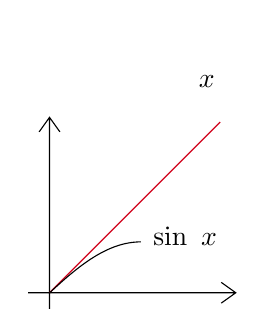
\begin{tikzpicture}[x=0.75pt,y=0.75pt,yscale=-1,xscale=1]
    %uncomment if require: \path (0,300); %set diagram left start at 0, and has height of 300
    
    %Shape: Axis 2D [id:dp008141030370613311] 
    \draw  (50,162.51) -- (150,162.51)(60.26,78) -- (60.26,178) (143,157.51) -- (150,162.51) -- (143,167.51) (55.26,85) -- (60.26,78) -- (65.26,85)  ;
    %Straight Lines [id:da3006663806705201] 
    \draw [color={rgb, 255:red, 208; green, 2; blue, 27 }  ,draw opacity=1 ]   (60.26,162.51) -- (142.51,80.26) ;
    %Shape: Wave [id:dp8304296493911976] 
    \draw   (104.26,138) .. controls (88.39,138) and (74.44,149.34) .. (60.26,162.59) ;
    
    % Text Node
    \draw (131,56.4) node [anchor=north west][inner sep=0.75pt]    {$x$};
    % Text Node
    \draw (109,129.4) node [anchor=north west][inner sep=0.75pt]    {$\sin \ x$};
    
    
    \end{tikzpicture}
    }
\begin{proof}
    Since $|\cos t|\leq 1$, \begin{align*}
        x-\sin x &= (x-\sin x)-(0-\sin 0)\\
        &= \int_{0}^{x}\underset{\geq 0}{\underbrace{1-\cos t}}\d t \qquad \text{by FTC}\\
        &\geq 0
    \end{align*}
\end{proof}

\proposition
In addition, $\cos x\geq 1-\frac{x^2}{2}$ for $x\geq 0$.\sidenote{These are the first 2 terms in the power series

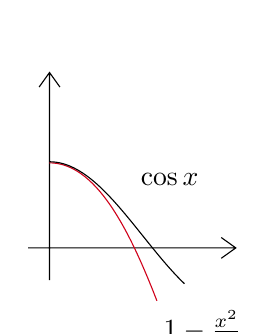
\begin{tikzpicture}[x=0.75pt,y=0.75pt,yscale=-1,xscale=1]
    %uncomment if require: \path (0,300); %set diagram left start at 0, and has height of 300
    
    %Shape: Axis 2D [id:dp008141030370613311] 
    \draw  (50,162.51) -- (150,162.51)(60.26,78) -- (60.26,178) (143,157.51) -- (150,162.51) -- (143,167.51) (55.26,85) -- (60.26,78) -- (65.26,85)  ;
    %Curve Lines [id:da027619260095050446] 
    \draw [color={rgb, 255:red, 208; green, 2; blue, 27 }  ,draw opacity=1 ]   (60.13,121.51) .. controls (82.26,121.51) and (98.26,152.51) .. (112,188) ;
    %Shape: Wave [id:dp87403708438032] 
    \draw   (60.26,121) .. controls (76.54,121) and (90.58,138.44) .. (105.26,156.76) .. controls (111.96,165.13) and (118.54,173.32) .. (125.26,179.74) ;
    
    % Text Node
    \draw (114,191.4) node [anchor=north west][inner sep=0.75pt]    {$1-\frac{x^{2}}{2}$};
    % Text Node
    \draw (103,125.4) node [anchor=north west][inner sep=0.75pt]    {$\cos x$};
    
    
    \end{tikzpicture}
    }
\begin{proof}
    The previous prop gives:
    \begin{align*}
        \cos x -1 &= \cos x -\cos 0\\
        &= \int_{0}^{x}-\sin t\d t\\
        &\geq \int_{0}^{x}- t\d t\\
        &= \frac{-x^2}{2}
    \end{align*}
\end{proof}

\proposition Furthermore, for $x\geq 0$: \begin{itemize}
    \item $\sin x\geq x^3-\frac{x^3}{6}$
    \item $\cos x\leq 1-\frac{x^2}{2}+\frac{x^4}{24}$
\end{itemize}

\begin{proposition}
    There exists $x_0\in (0,\sqrt{3})$ such that $\cos x_0=0$.
   \[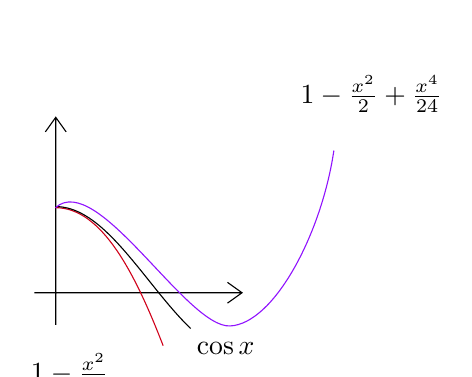
\begin{tikzpicture}[x=0.75pt,y=0.75pt,yscale=-1,xscale=1]
    %uncomment if require: \path (0,300); %set diagram left start at 0, and has height of 300
    
    %Shape: Axis 2D [id:dp008141030370613311] 
    \draw  (50,162.51) -- (150,162.51)(60.26,78) -- (60.26,178) (143,157.51) -- (150,162.51) -- (143,167.51) (55.26,85) -- (60.26,78) -- (65.26,85)  ;
    %Curve Lines [id:da027619260095050446] 
    \draw [color={rgb, 255:red, 208; green, 2; blue, 27 }  ,draw opacity=1 ]   (60.13,121.51) .. controls (82.26,121.51) and (98.26,152.51) .. (112,188) ;
    %Shape: Wave [id:dp87403708438032] 
    \draw   (60.26,121) .. controls (76.54,121) and (90.58,138.44) .. (105.26,156.76) .. controls (111.96,165.13) and (118.54,173.32) .. (125.26,179.74) ;
    %Curve Lines [id:da00092922647570437] 
    \draw [color={rgb, 255:red, 144; green, 19; blue, 254 }  ,draw opacity=1 ]   (60.13,121.51) .. controls (80.26,103.51) and (123.26,179.51) .. (144.26,178.51) .. controls (165.26,177.51) and (188.26,134.51) .. (194.26,94) ;
    
    % Text Node
    \draw (47,190.4) node [anchor=north west][inner sep=0.75pt]    {$1-\frac{x^{2}}{2}$};
    % Text Node
    \draw (127,185.4) node [anchor=north west][inner sep=0.75pt]    {$\cos x$};
    % Text Node
    \draw (177,56.4) node [anchor=north west][inner sep=0.75pt]    {$1-\frac{x^{2}}{2} +\frac{x^{4}}{24}$};
    
    
    \end{tikzpicture}
    \]
\end{proposition}
\begin{proof}
    By the previous prop, we have $\cos \sqrt{3}\leq  1-\frac{\sqrt 3^2}{2}+\frac{\sqrt 3^4}{24}=\frac{1}{8}< 0$. Moreover, $\cos 0=1>0$, by IVT, there exists $x_0\in (0,\sqrt{3})$ such that $\cos x_0=0$.
\end{proof}

\begin{proposition}
    $\omega_0=4x_0$ is a period of $e^{iz}$. 
\end{proposition}
\begin{proof}
    Since $\cos x_0=0$, we have $\sin x_0=\pm 1$. Then $e^{ix_0}=\pm i$. We have $(\pm i)^4=1$, so $e^{4ix_0}=1=e^{0}$, so $\omega_0=4x_0$ is a period of $e^{iz}$.
\end{proof}

\begin{proposition}
    $\omega_0$ is the \textit{smallest} positive period of $e^{iz}$.
\end{proposition}

\begin{proposition}
    All periods of $e^{iz}$ are integer multiples of $2\pi=4x_0$.
\end{proposition}

\begin{proof}
    Define $\pi=2x_0$. The area of unit circle is \begin{align*}
        4\int_{0}^{1}\sqrt{1-x^2}\d x &= 4\int_{0}^{\frac{\pi}{2}}\sqrt{1-\sin^2 \theta}\d \theta\\
        &= 4\int_{0}^{\frac{\pi}{2}}\frac{1}{2}(1+\cos 2\theta)\d \theta\\
        &= \pi
    \end{align*}
\end{proof}

\subsection{Complex logarithm}
We know: $e^0=1,e^1=\sum_{n=0}^{\infty}\frac{1}{n!}=2.718\dots$

Since $\frac{\d}{\d x}e^x=e^x$, it is positive. If $x>0$, we conclude that $e^x$ is strictly increasing! As $e^x=\sum_{n=0}^{\infty}\frac{x^n}{n!}>1+x$, so $\lim_{x\to \infty}e^x=\infty$,

Therefore, $e^x$ is a \textbf{bijection} from $\R$ to $(0,\infty)$. This means it has an inverse that is a bijection from $(0,\infty)$ to $\R$.

\defn $\ln x$ is the inverse of $e^x$ for $x\in (0,+\infty)$.

Now what about the complex case? Let $z\neq 0$ and $z=re^{i\theta}$\sidenote{cf. trig properties} where $r=|z|>0$ and $\theta=\arg z\in \R$.\sidenote{Only determined up to addition of multiples of $2\pi$}

Hence, $z=re^{i\theta}=e^{\ln r}e^{i\theta}=e^{\ln r+i\theta}$. However, the $\theta$ is ambiguous to addition of multiples of $2\pi$!

\addlink{Logarithm}
\defn If $z\neq 0$, a \textbf{logarithm} of $z$ is a $w\in \C$ such that $e^{w}=z$.

We could graph the function $e^z$ with $z\in \C$:       
\[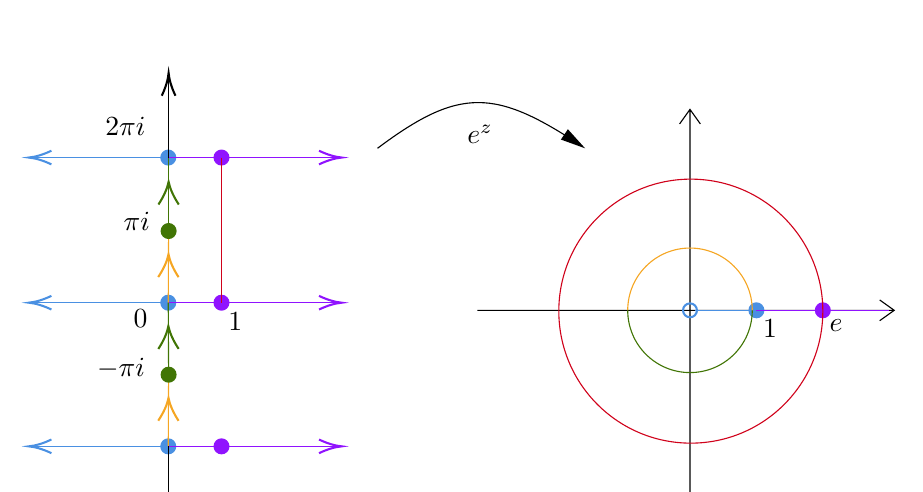
\begin{tikzpicture}[x=0.75pt,y=0.75pt,yscale=-1,xscale=1]
    %uncomment if require: \path (0,300); %set diagram left start at 0, and has height of 300
    
    %Straight Lines [id:da8785590871760756] 
    \draw [color={rgb, 255:red, 144; green, 19; blue, 254 }  ,draw opacity=1 ]   (145.63,130.39) -- (201.55,130.39) ;
    \draw [shift={(203.55,130.39)}, rotate = 180] [color={rgb, 255:red, 144; green, 19; blue, 254 }  ,draw opacity=1 ][line width=0.75]    (10.93,-3.29) .. controls (6.95,-1.4) and (3.31,-0.3) .. (0,0) .. controls (3.31,0.3) and (6.95,1.4) .. (10.93,3.29)   ;
    %Straight Lines [id:da1618236675525775] 
    \draw [color={rgb, 255:red, 74; green, 144; blue, 226 }  ,draw opacity=1 ]   (119.98,130.39) -- (54.75,130.39) ;
    \draw [shift={(52.75,130.39)}, rotate = 360] [color={rgb, 255:red, 74; green, 144; blue, 226 }  ,draw opacity=1 ][line width=0.75]    (10.93,-3.29) .. controls (6.95,-1.4) and (3.31,-0.3) .. (0,0) .. controls (3.31,0.3) and (6.95,1.4) .. (10.93,3.29)   ;
    \draw [shift={(119.98,130.39)}, rotate = 180] [color={rgb, 255:red, 74; green, 144; blue, 226 }  ,draw opacity=1 ][fill={rgb, 255:red, 74; green, 144; blue, 226 }  ,fill opacity=1 ][line width=0.75]      (0, 0) circle [x radius= 3.35, y radius= 3.35]   ;
    %Straight Lines [id:da8267712506988469] 
    \draw [color={rgb, 255:red, 144; green, 19; blue, 254 }  ,draw opacity=1 ]   (119.98,130.39) -- (145.63,130.39) ;
    \draw [shift={(145.63,130.39)}, rotate = 0] [color={rgb, 255:red, 144; green, 19; blue, 254 }  ,draw opacity=1 ][fill={rgb, 255:red, 144; green, 19; blue, 254 }  ,fill opacity=1 ][line width=0.75]      (0, 0) circle [x radius= 3.35, y radius= 3.35]   ;
    %Straight Lines [id:da2374921790479616] 
    \draw [color={rgb, 255:red, 144; green, 19; blue, 254 }  ,draw opacity=1 ]   (145.63,199.6) -- (201.55,199.6) ;
    \draw [shift={(203.55,199.6)}, rotate = 180] [color={rgb, 255:red, 144; green, 19; blue, 254 }  ,draw opacity=1 ][line width=0.75]    (10.93,-3.29) .. controls (6.95,-1.4) and (3.31,-0.3) .. (0,0) .. controls (3.31,0.3) and (6.95,1.4) .. (10.93,3.29)   ;
    %Straight Lines [id:da03468902350963088] 
    \draw [color={rgb, 255:red, 74; green, 144; blue, 226 }  ,draw opacity=1 ]   (119.98,199.6) -- (54.75,199.6) ;
    \draw [shift={(52.75,199.6)}, rotate = 360] [color={rgb, 255:red, 74; green, 144; blue, 226 }  ,draw opacity=1 ][line width=0.75]    (10.93,-3.29) .. controls (6.95,-1.4) and (3.31,-0.3) .. (0,0) .. controls (3.31,0.3) and (6.95,1.4) .. (10.93,3.29)   ;
    \draw [shift={(119.98,199.6)}, rotate = 180] [color={rgb, 255:red, 74; green, 144; blue, 226 }  ,draw opacity=1 ][fill={rgb, 255:red, 74; green, 144; blue, 226 }  ,fill opacity=1 ][line width=0.75]      (0, 0) circle [x radius= 3.35, y radius= 3.35]   ;
    %Straight Lines [id:da3208922622885413] 
    \draw [color={rgb, 255:red, 144; green, 19; blue, 254 }  ,draw opacity=1 ]   (119.98,199.6) -- (145.63,199.6) ;
    \draw [shift={(145.63,199.6)}, rotate = 0] [color={rgb, 255:red, 144; green, 19; blue, 254 }  ,draw opacity=1 ][fill={rgb, 255:red, 144; green, 19; blue, 254 }  ,fill opacity=1 ][line width=0.75]      (0, 0) circle [x radius= 3.35, y radius= 3.35]   ;
    %Straight Lines [id:da4709032693595072] 
    \draw [color={rgb, 255:red, 144; green, 19; blue, 254 }  ,draw opacity=1 ]   (145.63,60.46) -- (201.55,60.46) ;
    \draw [shift={(203.55,60.46)}, rotate = 180] [color={rgb, 255:red, 144; green, 19; blue, 254 }  ,draw opacity=1 ][line width=0.75]    (10.93,-3.29) .. controls (6.95,-1.4) and (3.31,-0.3) .. (0,0) .. controls (3.31,0.3) and (6.95,1.4) .. (10.93,3.29)   ;
    %Straight Lines [id:da05828217640270972] 
    \draw [color={rgb, 255:red, 74; green, 144; blue, 226 }  ,draw opacity=1 ]   (119.98,60.46) -- (54.75,60.46) ;
    \draw [shift={(52.75,60.46)}, rotate = 360] [color={rgb, 255:red, 74; green, 144; blue, 226 }  ,draw opacity=1 ][line width=0.75]    (10.93,-3.29) .. controls (6.95,-1.4) and (3.31,-0.3) .. (0,0) .. controls (3.31,0.3) and (6.95,1.4) .. (10.93,3.29)   ;
    \draw [shift={(119.98,60.46)}, rotate = 180] [color={rgb, 255:red, 74; green, 144; blue, 226 }  ,draw opacity=1 ][fill={rgb, 255:red, 74; green, 144; blue, 226 }  ,fill opacity=1 ][line width=0.75]      (0, 0) circle [x radius= 3.35, y radius= 3.35]   ;
    %Straight Lines [id:da6226539504724369] 
    \draw [color={rgb, 255:red, 144; green, 19; blue, 254 }  ,draw opacity=1 ]   (119.98,60.46) -- (145.63,60.46) ;
    \draw [shift={(145.63,60.46)}, rotate = 0] [color={rgb, 255:red, 144; green, 19; blue, 254 }  ,draw opacity=1 ][fill={rgb, 255:red, 144; green, 19; blue, 254 }  ,fill opacity=1 ][line width=0.75]      (0, 0) circle [x radius= 3.35, y radius= 3.35]   ;
    %Straight Lines [id:da35528692959663144] 
    \draw [color={rgb, 255:red, 245; green, 166; blue, 35 }  ,draw opacity=1 ]   (119.98,130.39) -- (120.15,95.86) ;
    \draw [shift={(120.1,107.13)}, rotate = 90.28] [color={rgb, 255:red, 245; green, 166; blue, 35 }  ,draw opacity=1 ][line width=0.75]    (10.93,-4.9) .. controls (6.95,-2.3) and (3.31,-0.67) .. (0,0) .. controls (3.31,0.67) and (6.95,2.3) .. (10.93,4.9)   ;
    %Straight Lines [id:da8648044267590989] 
    \draw [color={rgb, 255:red, 65; green, 117; blue, 5 }  ,draw opacity=1 ]   (120.15,95.86) -- (120.15,60.46) ;
    \draw [shift={(120.15,72.16)}, rotate = 90] [color={rgb, 255:red, 65; green, 117; blue, 5 }  ,draw opacity=1 ][line width=0.75]    (10.93,-4.9) .. controls (6.95,-2.3) and (3.31,-0.67) .. (0,0) .. controls (3.31,0.67) and (6.95,2.3) .. (10.93,4.9)   ;
    \draw [shift={(120.15,95.86)}, rotate = 270] [color={rgb, 255:red, 65; green, 117; blue, 5 }  ,draw opacity=1 ][fill={rgb, 255:red, 65; green, 117; blue, 5 }  ,fill opacity=1 ][line width=0.75]      (0, 0) circle [x radius= 3.35, y radius= 3.35]   ;
    %Straight Lines [id:da878911184832804] 
    \draw [color={rgb, 255:red, 245; green, 166; blue, 35 }  ,draw opacity=1 ]   (119.98,199.6) -- (120.15,165.07) ;
    \draw [shift={(120.1,176.34)}, rotate = 90.28] [color={rgb, 255:red, 245; green, 166; blue, 35 }  ,draw opacity=1 ][line width=0.75]    (10.93,-4.9) .. controls (6.95,-2.3) and (3.31,-0.67) .. (0,0) .. controls (3.31,0.67) and (6.95,2.3) .. (10.93,4.9)   ;
    %Straight Lines [id:da0013946467543932695] 
    \draw [color={rgb, 255:red, 65; green, 117; blue, 5 }  ,draw opacity=1 ]   (120.15,165.07) -- (119.98,130.39) ;
    \draw [shift={(120.04,141.73)}, rotate = 89.72] [color={rgb, 255:red, 65; green, 117; blue, 5 }  ,draw opacity=1 ][line width=0.75]    (10.93,-4.9) .. controls (6.95,-2.3) and (3.31,-0.67) .. (0,0) .. controls (3.31,0.67) and (6.95,2.3) .. (10.93,4.9)   ;
    \draw [shift={(120.15,165.07)}, rotate = 269.72] [color={rgb, 255:red, 65; green, 117; blue, 5 }  ,draw opacity=1 ][fill={rgb, 255:red, 65; green, 117; blue, 5 }  ,fill opacity=1 ][line width=0.75]      (0, 0) circle [x radius= 3.35, y radius= 3.35]   ;
    %Straight Lines [id:da6431192925230409] 
    \draw    (120.15,60.46) -- (120.15,21.72) ;
    \draw [shift={(120.15,19.72)}, rotate = 90] [color={rgb, 255:red, 0; green, 0; blue, 0 }  ][line width=0.75]    (10.93,-3.29) .. controls (6.95,-1.4) and (3.31,-0.3) .. (0,0) .. controls (3.31,0.3) and (6.95,1.4) .. (10.93,3.29)   ;
    %Straight Lines [id:da4817110891560017] 
    \draw    (119.98,225.34) -- (119.98,199.6) ;
    %Curve Lines [id:da15130320225307914] 
    \draw    (220.8,56) .. controls (260.4,26.3) and (277.71,27.23) .. (319.53,55.15) ;
    \draw [shift={(320.8,56)}, rotate = 213.92] [fill={rgb, 255:red, 0; green, 0; blue, 0 }  ][line width=0.08]  [draw opacity=0] (12,-3) -- (0,0) -- (12,3) -- cycle    ;
    %Shape: Axis 2D [id:dp10703039654547442] 
    \draw  (268.95,134.06) -- (469.75,134.06)(371.35,37.26) -- (371.35,229.26) (462.75,129.06) -- (469.75,134.06) -- (462.75,139.06) (366.35,44.26) -- (371.35,37.26) -- (376.35,44.26)  ;
    %Straight Lines [id:da39023709471268675] 
    \draw [color={rgb, 255:red, 74; green, 144; blue, 226 }  ,draw opacity=1 ]   (373.7,134.06) -- (403.35,134.06) ;
    \draw [shift={(403.35,134.06)}, rotate = 0] [color={rgb, 255:red, 74; green, 144; blue, 226 }  ,draw opacity=1 ][fill={rgb, 255:red, 74; green, 144; blue, 226 }  ,fill opacity=1 ][line width=0.75]      (0, 0) circle [x radius= 3.35, y radius= 3.35]   ;
    \draw [shift={(371.35,134.06)}, rotate = 0] [color={rgb, 255:red, 74; green, 144; blue, 226 }  ,draw opacity=1 ][line width=0.75]      (0, 0) circle [x radius= 3.35, y radius= 3.35]   ;
    %Straight Lines [id:da20992201553768708] 
    \draw [color={rgb, 255:red, 144; green, 19; blue, 254 }  ,draw opacity=1 ]   (435.35,134.06) -- (467.35,134.06) ;
    \draw [shift={(435.35,134.06)}, rotate = 0] [color={rgb, 255:red, 144; green, 19; blue, 254 }  ,draw opacity=1 ][fill={rgb, 255:red, 144; green, 19; blue, 254 }  ,fill opacity=1 ][line width=0.75]      (0, 0) circle [x radius= 3.35, y radius= 3.35]   ;
    %Straight Lines [id:da895300882766211] 
    \draw [color={rgb, 255:red, 144; green, 19; blue, 254 }  ,draw opacity=1 ]   (403.35,134.06) -- (435.35,134.06) ;
    %Shape: Arc [id:dp17152249012602994] 
    \draw  [draw opacity=0] (341.35,134.06) .. controls (341.35,134.06) and (341.35,134.06) .. (341.35,134.06) .. controls (341.35,117.49) and (354.78,104.06) .. (371.35,104.06) .. controls (387.92,104.06) and (401.35,117.49) .. (401.35,134.06) .. controls (401.35,134.06) and (401.35,134.06) .. (401.35,134.06) -- (371.35,134.06) -- cycle ; \draw [color={rgb, 255:red, 245; green, 166; blue, 35 }  ,draw opacity=1 ]   (341.35,134.06) .. controls (341.35,117.49) and (354.78,104.06) .. (371.35,104.06) .. controls (387.92,104.06) and (401.35,117.49) .. (401.35,134.06) ;  
    %Shape: Arc [id:dp054572774151422365] 
    \draw  [draw opacity=0] (401.35,134.06) .. controls (401.35,134.06) and (401.35,134.06) .. (401.35,134.06) .. controls (401.35,150.63) and (387.92,164.06) .. (371.35,164.06) .. controls (354.78,164.06) and (341.35,150.63) .. (341.35,134.06) .. controls (341.35,134.06) and (341.35,134.06) .. (341.35,134.06) -- (371.35,134.06) -- cycle ; \draw [color={rgb, 255:red, 65; green, 117; blue, 5 }  ,draw opacity=1 ]   (401.35,134.06) .. controls (401.35,150.63) and (387.92,164.06) .. (371.35,164.06) .. controls (354.78,164.06) and (341.35,150.63) .. (341.35,134.06) ;  
    %Straight Lines [id:da7090062681421083] 
    \draw [color={rgb, 255:red, 208; green, 2; blue, 27 }  ,draw opacity=1 ]   (145.63,60.46) -- (145.63,130.39) ;
    %Shape: Circle [id:dp2705523730959791] 
    \draw  [color={rgb, 255:red, 208; green, 2; blue, 27 }  ,draw opacity=1 ] (308.15,134.46) .. controls (308.15,99.34) and (336.63,70.86) .. (371.75,70.86) .. controls (406.88,70.86) and (435.35,99.34) .. (435.35,134.46) .. controls (435.35,169.59) and (406.88,198.06) .. (371.75,198.06) .. controls (336.63,198.06) and (308.15,169.59) .. (308.15,134.46) -- cycle ;
    
    % Text Node
    \draw (102,132.4) node [anchor=north west][inner sep=0.75pt]    {$0$};
    % Text Node
    \draw (147.63,133.79) node [anchor=north west][inner sep=0.75pt]    {$1$};
    % Text Node
    \draw (88.4,40) node [anchor=north west][inner sep=0.75pt]    {$2\pi i$};
    % Text Node
    \draw (97.2,85.6) node [anchor=north west][inner sep=0.75pt]    {$\pi i$};
    % Text Node
    \draw (84.4,156) node [anchor=north west][inner sep=0.75pt]    {$-\pi i$};
    % Text Node
    \draw (262.8,43.4) node [anchor=north west][inner sep=0.75pt]    {$e^{z}$};
    % Text Node
    \draw (405.35,137.46) node [anchor=north west][inner sep=0.75pt]    {$1$};
    % Text Node
    \draw (437.35,137.46) node [anchor=north west][inner sep=0.75pt]    {$e$};
    
    
    \end{tikzpicture}
    \]

\defn If $\Omega$ is a region in $\C$, then a continuous $l:\Omega \to \C$ is a \textbf{branch} of the logarithm if $e^{l(z)}=z$ for all $z\in \Omega$.\sidenote{note $0\notin \Omega$}

\addlink{Principal branch of the logarithm}
\eg If $\Omega=\C\backslash(-\infty, 0]$ such that $\theta\in (-\pi,\pi)$, a logarithm could be defined on it. This is the \textbf{principal branch} of the logarithm.\sidenote{See \href{https://stephangarcia.sites.pomona.edu/teaching/24S-135/Lecture/24S-135-Lecture10.pdf}{graphed Riemann surface}}

\addlink{First derivative of ln}
\rmk Suppose $l(z)$ is a branch of the logarithm and $l$ is analytic, then: \[e^{l(z)}=z\implies \frac{\d}{\d z}e^{l(z)} = l'(z)e^{l(z)}=1\]

Since $e^{l(z)}=z$, we conclude $l'(z)=\frac{1}{z}$.

\subsection{Complex power}
\defn If $z\neq 0$, \textit{define} $z^{a}=e^{a\log z}$.\sidenote{NOT well-defined!}

\rmk The definition of complex powers should coincide with the old one: $z^n=\underset{n}{\underbrace{z\cdot z\cdot\dots\cdot z}=r^ne^{in\theta}}$.

Check: \begin{align*}
    z^n&=e^{n\log z}=e^{n(\ln r+i\theta+i2\pi k)}\\
    &= e^{n\ln r}e^{in\theta}\underset{=1}{\underbrace{e^{i2\pi nk}}}\\
    &= r^ne^{in\theta}
\end{align*} is true for any $k\in \Z$.

How about $n$-th roots?
\begin{align*}
    z^{\frac{1}{n}} &= e^{\frac{1}{n}\log z}\\
    &= e^{\frac{1}{n}(\ln r+i\theta+i2\pi k)}\\
    &= e^{\frac{1}{n}\ln r}e^{\frac{i\theta}{n}}\underset{\text{$n$ distinct}}{\underbrace{e^{\frac{i2\pi k}{n}}}}\\
    &= r^{\frac{1}{n}} e^{i\left(\frac{\theta+2\pi k}{n}\right)}
\end{align*}

\subsection{Riemann surface}
We still have a problem: $\ln z$ is still not a function on $\C$! The branch depends on the arbitrary choice of domain. What shall we do to make it not dependent on a choice?

Answer: let $\ln$ not live on the complex plane, but  infinitely many copies of the slit plane $\C\backslash(-\infty, 0]$, each
one being glued to the next along the slit $(-\infty, 0]$.

\eg $z^{1/2}$ would live on a surface:
\[\begin{tikzpicture}[x=0.75pt,y=0.75pt,yscale=-1,xscale=1]
    %uncomment if require: \path (0,300); %set diagram left start at 0, and has height of 300
    
    %Straight Lines [id:da9680702032506614] 
    \draw [color={rgb, 255:red, 208; green, 2; blue, 27 }  ,draw opacity=1 ] [dash pattern={on 4.5pt off 4.5pt}]  (124.85,130) -- (33.35,130) ;
    \draw [shift={(31.35,130)}, rotate = 360] [color={rgb, 255:red, 208; green, 2; blue, 27 }  ,draw opacity=1 ][line width=0.75]    (10.93,-3.29) .. controls (6.95,-1.4) and (3.31,-0.3) .. (0,0) .. controls (3.31,0.3) and (6.95,1.4) .. (10.93,3.29)   ;
    \draw [shift={(127.2,130)}, rotate = 180] [color={rgb, 255:red, 208; green, 2; blue, 27 }  ,draw opacity=1 ][line width=0.75]      (0, 0) circle [x radius= 3.35, y radius= 3.35]   ;
    %Shape: Arc [id:dp6906978961263923] 
    \draw  [draw opacity=0] (86.68,130) .. controls (86.68,130) and (86.68,130) .. (86.68,130) .. controls (86.68,107.62) and (104.82,89.48) .. (127.2,89.48) .. controls (149.58,89.48) and (167.72,107.62) .. (167.72,130) -- (127.2,130) -- cycle ; \draw [color={rgb, 255:red, 245; green, 166; blue, 35 }  ,draw opacity=1 ]   (86.68,130) .. controls (86.68,130) and (86.68,130) .. (86.68,130) .. controls (86.68,107.62) and (104.82,89.48) .. (127.2,89.48) .. controls (149.58,89.48) and (167.72,107.62) .. (167.72,130) ;  
    %Shape: Arc [id:dp9861691627816211] 
    \draw  [draw opacity=0] (167.72,130) .. controls (167.72,130) and (167.72,130) .. (167.72,130) .. controls (167.72,152.38) and (149.58,170.52) .. (127.2,170.52) .. controls (104.82,170.52) and (86.68,152.38) .. (86.68,130) -- (127.2,130) -- cycle ; \draw [color={rgb, 255:red, 65; green, 117; blue, 5 }  ,draw opacity=1 ]   (167.72,130) .. controls (167.72,130) and (167.72,130) .. (167.72,130) .. controls (167.72,152.38) and (149.58,170.52) .. (127.2,170.52) .. controls (104.82,170.52) and (86.68,152.38) .. (86.68,130) ;  
    %Straight Lines [id:da9124411332810323] 
    \draw [color={rgb, 255:red, 208; green, 2; blue, 27 }  ,draw opacity=1 ] [dash pattern={on 4.5pt off 4.5pt}]  (318.45,130) -- (226.95,130) ;
    \draw [shift={(224.95,130)}, rotate = 360] [color={rgb, 255:red, 208; green, 2; blue, 27 }  ,draw opacity=1 ][line width=0.75]    (10.93,-3.29) .. controls (6.95,-1.4) and (3.31,-0.3) .. (0,0) .. controls (3.31,0.3) and (6.95,1.4) .. (10.93,3.29)   ;
    \draw [shift={(320.8,130)}, rotate = 180] [color={rgb, 255:red, 208; green, 2; blue, 27 }  ,draw opacity=1 ][line width=0.75]      (0, 0) circle [x radius= 3.35, y radius= 3.35]   ;
    %Shape: Arc [id:dp05520981510099365] 
    \draw  [draw opacity=0] (280.28,130) .. controls (280.28,107.62) and (298.42,89.48) .. (320.8,89.48) .. controls (343.18,89.48) and (361.32,107.62) .. (361.32,130) -- (320.8,130) -- cycle ; \draw [color={rgb, 255:red, 65; green, 117; blue, 5 }  ,draw opacity=1 ]   (280.28,130) .. controls (280.28,107.62) and (298.42,89.48) .. (320.8,89.48) .. controls (343.18,89.48) and (361.32,107.62) .. (361.32,130) ;  
    %Shape: Arc [id:dp5073887586255386] 
    \draw  [draw opacity=0] (361.32,130) .. controls (361.32,130) and (361.32,130) .. (361.32,130) .. controls (361.32,130) and (361.32,130) .. (361.32,130) .. controls (361.32,152.38) and (343.18,170.52) .. (320.8,170.52) .. controls (298.42,170.52) and (280.28,152.38) .. (280.28,130) -- (320.8,130) -- cycle ; \draw [color={rgb, 255:red, 245; green, 166; blue, 35 }  ,draw opacity=1 ]   (361.32,130) .. controls (361.32,130) and (361.32,130) .. (361.32,130) .. controls (361.32,152.38) and (343.18,170.52) .. (320.8,170.52) .. controls (298.42,170.52) and (280.28,152.38) .. (280.28,130) ;  
    
    % Text Node
    \draw (171.6,124.6) node [anchor=north west][inner sep=0.75pt]    {$1$};
    % Text Node
    \draw (70.8,109.2) node [anchor=north west][inner sep=0.75pt]    {$i$};
    % Text Node
    \draw (367.6,122.8) node [anchor=north west][inner sep=0.75pt]    {$-1$};
    % Text Node
    \draw (258.8,106.8) node [anchor=north west][inner sep=0.75pt]    {$-i$};
    
    
    \end{tikzpicture}
    \]

\section{Cauchy's theorem and its consequences}

\subsection{Complex integration}
\addlink{Piecewise continuity}
\defn A complex-valued function $\gamma:[a,b]\to \C$ is \textbf{piecewise} continuous if $\gamma$ is continuous at all but \textit{finitely many} points of $[a,b]$ and $\gamma$ has one-sided limits that are \textit{finite} at each point (of discontinuity).

\[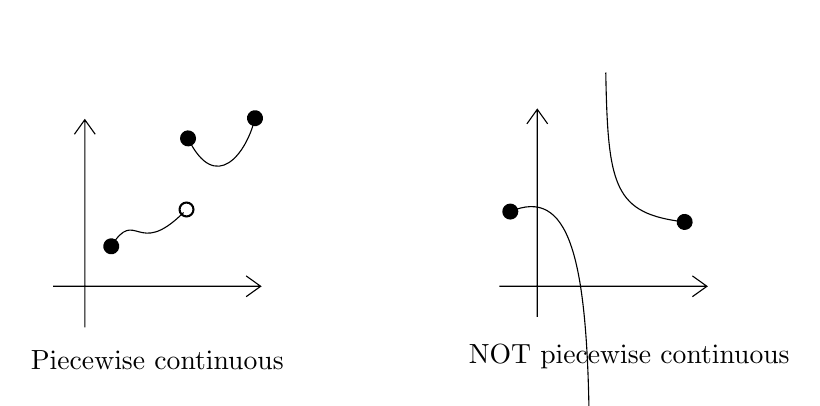
\begin{tikzpicture}[x=0.75pt,y=0.75pt,yscale=-1,xscale=1]
    %uncomment if require: \path (0,300); %set diagram left start at 0, and has height of 300
    
    %Shape: Axis 2D [id:dp7003951674563056] 
    \draw  (50,158.26) -- (150,158.26)(65.26,78) -- (65.26,178) (143,153.26) -- (150,158.26) -- (143,163.26) (60.26,85) -- (65.26,78) -- (70.26,85)  ;
    %Curve Lines [id:da5314714499980906] 
    \draw    (78,139) .. controls (90.01,119.66) and (90.25,145.2) .. (112.84,122.7) ;
    \draw [shift={(114.26,121.26)}, rotate = 313.83] [color={rgb, 255:red, 0; green, 0; blue, 0 }  ][line width=0.75]      (0, 0) circle [x radius= 3.35, y radius= 3.35]   ;
    \draw [shift={(78,139)}, rotate = 301.84] [color={rgb, 255:red, 0; green, 0; blue, 0 }  ][fill={rgb, 255:red, 0; green, 0; blue, 0 }  ][line width=0.75]      (0, 0) circle [x radius= 3.35, y radius= 3.35]   ;
    %Curve Lines [id:da27910409809362413] 
    \draw    (115,87) .. controls (128.26,114.26) and (143.26,94.26) .. (147.26,77.26) ;
    \draw [shift={(147.26,77.26)}, rotate = 283.24] [color={rgb, 255:red, 0; green, 0; blue, 0 }  ][fill={rgb, 255:red, 0; green, 0; blue, 0 }  ][line width=0.75]      (0, 0) circle [x radius= 3.35, y radius= 3.35]   ;
    \draw [shift={(115,87)}, rotate = 64.07] [color={rgb, 255:red, 0; green, 0; blue, 0 }  ][fill={rgb, 255:red, 0; green, 0; blue, 0 }  ][line width=0.75]      (0, 0) circle [x radius= 3.35, y radius= 3.35]   ;
    %Shape: Axis 2D [id:dp8923800564332263] 
    \draw  (265,158.26) -- (365,158.26)(283.26,73) -- (283.26,173) (358,153.26) -- (365,158.26) -- (358,163.26) (278.26,80) -- (283.26,73) -- (288.26,80)  ;
    %Curve Lines [id:da7330323189044972] 
    \draw    (270.26,122.26) .. controls (298.26,110.26) and (307.26,143.26) .. (308.26,223.26) ;
    \draw [shift={(270.26,122.26)}, rotate = 336.8] [color={rgb, 255:red, 0; green, 0; blue, 0 }  ][fill={rgb, 255:red, 0; green, 0; blue, 0 }  ][line width=0.75]      (0, 0) circle [x radius= 3.35, y radius= 3.35]   ;
    %Curve Lines [id:da7451055597374061] 
    \draw    (354.26,127.26) .. controls (320.26,123.26) and (317.26,110.26) .. (316.26,55.26) ;
    \draw [shift={(354.26,127.26)}, rotate = 186.71] [color={rgb, 255:red, 0; green, 0; blue, 0 }  ][fill={rgb, 255:red, 0; green, 0; blue, 0 }  ][line width=0.75]      (0, 0) circle [x radius= 3.35, y radius= 3.35]   ;
    
    % Text Node
    \draw (38,188) node [anchor=north west][inner sep=0.75pt]   [align=left] {Piecewise continuous};
    % Text Node
    \draw (249,185) node [anchor=north west][inner sep=0.75pt]   [align=left] {NOT piecewise continuous};
    
    
    \end{tikzpicture}\]

If $\gamma$ is piecewise continuous, then $\int_{a}^{b}\re \gamma(t)\d t$ and $\int_{a}^{b}\im \gamma(t)\d t$ exist. Then we define \textbf{complex integration}:
\[\int_{a}^{b}\gamma(t)\d t = \int_{a}^{b}\re \gamma(t)\d t +i\cdot \int_{a}^{b}\im \gamma(t)\d t\]

That is, \begin{align*}
    \re \left(\int_{a}^{b}\gamma(t)\d t\right)&=\int_{a}^{b}\re \gamma(t)\d t\\
    \im \left(\int_{a}^{b}\gamma(t)\d t\right)&=\int_{a}^{b}\im \gamma(t)\d t\\
\end{align*}

In addition, if $\gamma_1,\gamma_2$ are both $[a,b]\to \C$ and piecewise cont., and $c_1,c_2\in\C$, then \[\int_{a}^{b}\left( c_1\gamma_1(t)+c_2\gamma_2(t) \right)\d t=c_1\int_{a}^{b}\gamma_1(t)\d t+c_2\int_{a}^{b}\gamma_2(t)\d t\]

\addlink{Triangle inequality}
\begin{proposition}[Triangle inequality]
    If $\gamma:[a,b]\to \C$ is {piecewise} continuous, then \[\left|\int_{a}^{b}\gamma(t)\d t \right|\leq \int_{a}^{b}|\gamma(t)|\d t \]
\end{proposition}
\begin{proof}
    WLOG assume $ \int_{a}^{b}\gamma(t)\d t \neq 0$. Define $\lambda = \frac{\left|\int_{a}^{b}\gamma(t)\d t\right|}{\int_{a}^{b}\gamma(t)\d t}$ and note $|\lambda|=1$.

    Thus, \begin{align*}
        \left|\int_{a}^{b}\gamma(t)\d t\right| &= \lambda\int_{a}^{b}\gamma(t)\d t\\
        &= \int_{a}^{b}\lambda\gamma(t)\d t &&\text{because LHS is }\in \R\\
        &= \re \int_{a}^{b}\lambda\gamma(t)\d t\\
        &\leq \int_{a}^{b}|\lambda\gamma(t)|\d t &&\because \re z\leq |z|\\
        &= \int_{a}^{b}|\gamma(t)|\d t&& \because |\lambda|=1
    \end{align*}
\end{proof}

\subsubsection{Complex differentiability}
\defn $\gamma:[a,b]\to \C$ is \textbf{differentiable} at $t\in [a,b]$ if $\re \gamma$ and $\im \gamma$ are differentiable (in the sense of real variables). We define \[\gamma'(t)=(\re \gamma)'(t)+i\cdot (\im \gamma)'(t)\]

\defn $\gamma:[a,b]\to \C$ is \textbf{piecewise} $C^1$\sidenote{$C^1$ is one-time differentiable} if: \begin{enumerate}[label=(\alph*)]
    \item $\gamma$ is continuous on $[a,b]$.
    \item $\gamma$ is differentiable at all but finitely many points of $[a,b]$.
    \item $\gamma'$ is continuous at each point where it exists.
    \item $\gamma'$ has finite one-sided limits at every point of discontinuity.
\end{enumerate}

\subsubsection{Fundamental theorem of calculus, complex edition}
If $\gamma:[a,b]\to\C$ is piecewise $C^1$, then:
\[\int_{a}^{b}\gamma'(t)\d t=\gamma(b)-\gamma(a)\]

\defn If $\gamma$ is $C^1$, then the arclength
\sidenote{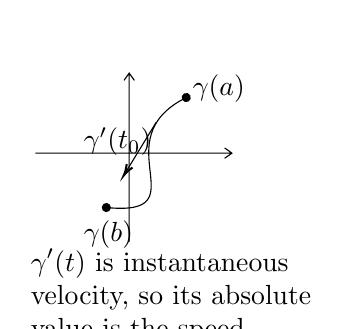
\begin{tikzpicture}[x=0.75pt,y=0.75pt,yscale=-0.5,xscale=0.5]
    %uncomment if require: \path (0,286); %set diagram left start at 0, and has height of 286
    
    %Shape: Axis 2D [id:dp5992461788507699] 
    \draw  (50,141.08) -- (239.26,141.08)(140.26,64) -- (140.26,226.51) (232.26,136.08) -- (239.26,141.08) -- (232.26,146.08) (135.26,71) -- (140.26,64) -- (145.26,71)  ;
    %Curve Lines [id:da8169369769076535] 
    \draw    (118.26,193.51) .. controls (210.26,202.51) and (113.26,128.51) .. (195.26,87.51) ;
    \draw [shift={(195.26,87.51)}, rotate = 333.43] [color={rgb, 255:red, 0; green, 0; blue, 0 }  ][fill={rgb, 255:red, 0; green, 0; blue, 0 }  ][line width=0.75]      (0, 0) circle [x radius= 3.35, y radius= 3.35]   ;
    \draw [shift={(118.26,193.51)}, rotate = 5.59] [color={rgb, 255:red, 0; green, 0; blue, 0 }  ][fill={rgb, 255:red, 0; green, 0; blue, 0 }  ][line width=0.75]      (0, 0) circle [x radius= 3.35, y radius= 3.35]   ;
    %Straight Lines [id:da7279313778056917] 
    \draw    (166.26,111.51) -- (136.05,160.92) ;
    \draw [shift={(135,162.63)}, rotate = 301.44] [color={rgb, 255:red, 0; green, 0; blue, 0 }  ][line width=0.75]    (10.93,-3.29) .. controls (6.95,-1.4) and (3.31,-0.3) .. (0,0) .. controls (3.31,0.3) and (6.95,1.4) .. (10.93,3.29)   ;
    
    % Text Node
    \draw (199,63.4) node [anchor=north west][inner sep=0.75pt]    {$\gamma ( a)$};
    % Text Node
    \draw (94,203.4) node [anchor=north west][inner sep=0.75pt]    {$\gamma ( b)$};
    % Text Node
    \draw (94,114.4) node [anchor=north west][inner sep=0.75pt]    {$\gamma '( t_{0})$};
    % Text Node
    \draw (43,231) node [anchor=north west][inner sep=0.75pt]   [align=left] {$\displaystyle \gamma '( t)$ is instantaneous\\ velocity, so its absolute\\ value is the speed};
    
    
    \end{tikzpicture}
    } 
    of $\gamma$ is: \[L(\gamma)=\int_{a}^{b}|\gamma'(t)|\d t\]

\defn If $\gamma:[a,b]\to \reg$ is piecewise $C^1$ and $f:\reg \to\C$ is continuous, then \[\int_{\gamma}f(z)\d z=\int_{a}^{b}f(\gamma(t))\gamma'(t)\d t\]
where $z=\gamma(t)$ and $\d z=\gamma'(t)\d t$

We have \textbf{linearity} w.r.t. $f$: \[\int_{\gamma}\left( c_1f_1(z)+c_2f_2(z) \right)\d z=c_1\int_{\gamma}f_1(z)\d z+c_2\int_{\gamma}f_2(z)\d z\]

\rmk Arclength is independent from parameterization.
\begin{proof}
    Let $\gamma:[a,b]\to \reg$ be piecewise $C^1$. Let $\alpha:[c,d] \to [a,b]$ is an increasing, piecewise $C^1$ surjection such that $\alpha(c)=a, \alpha(d)=b$. Then $\phi=\gamma\circ \alpha:[c,d]\to \reg$ is also piecewise $C^1$. Hence, by substituting $s=\alpha(t), \d s=\alpha'(t)\d t$:
    \begin{align*}
        \int_{\phi}f(z)\d z&=\int_{c}^{d}f(\phi(t))\phi'(t)\d t\\
        &= \int_{c}^{d}f(\gamma(\alpha(t)))\gamma'(\alpha(t))\alpha'(t)\d t\\
        &= \int_{a}^{b}f(\gamma(s))\gamma'(s)\d s\\
        &= \int_{\gamma}f(z)\d z
    \end{align*}
\end{proof}

\subsubsection{An important estimate}
Let $f$ be continuous. Since \(\int_{\gamma}f(z)\d z=\int_{a}^{b}f(\gamma(t))\gamma'(t)\d t\), we observe: \begin{align*}
    \left|\int_{\gamma}f(z)\d z\right|&=\left|\int_{a}^{b}f(\gamma(t))\gamma'(t)\d t\right|\\
    &\leq \int_{a}^{b}|f(\gamma(t))|\,|\gamma'(t)|\d t\\
    &\leq \max_{t\in [a,b]}|f(\gamma(t))| \int_{a}^{b}|\gamma'(t)|\d t\\
    &= \rt{\max_{z\in \gamma}|f(z)|\cdot L(\gamma)}
\end{align*}


\defn If $\gamma:[a,b]\to\C$, the reverse of $\gamma$ is $(-\gamma):[-b,-a]\to\C$ defined by $(-\gamma)(t)=\gamma(-t)$. \sidenote{going around the track backwards} Hence, \[\int_{-\gamma}f(z)\d z= -\int_{\gamma}f(z)\d z\]

\rmk We can also break up the curve and integral the two parts separately: \sidenote{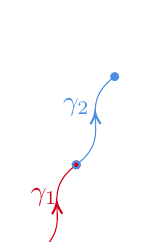
\begin{tikzpicture}[x=0.75pt,y=0.75pt,yscale=-0.5,xscale=0.5]
    %uncomment if require: \path (0,300); %set diagram left start at 0, and has height of 300
    
    %Curve Lines [id:da6510647213107017] 
    \draw [color={rgb, 255:red, 208; green, 2; blue, 27 }  ,draw opacity=1 ]   (144.26,215.76) .. controls (184.26,185.76) and (141.26,160.76) .. (181.26,130.76) ;
    \draw [shift={(181.26,130.76)}, rotate = 323.13] [color={rgb, 255:red, 208; green, 2; blue, 27 }  ,draw opacity=1 ][fill={rgb, 255:red, 208; green, 2; blue, 27 }  ,fill opacity=1 ][line width=0.75]      (0, 0) circle [x radius= 3.35, y radius= 3.35]   ;
    \draw [shift={(162.49,167.07)}, rotate = 87.57] [color={rgb, 255:red, 208; green, 2; blue, 27 }  ,draw opacity=1 ][line width=0.75]    (10.93,-4.9) .. controls (6.95,-2.3) and (3.31,-0.67) .. (0,0) .. controls (3.31,0.67) and (6.95,2.3) .. (10.93,4.9)   ;
    \draw [shift={(144.26,215.76)}, rotate = 323.13] [color={rgb, 255:red, 208; green, 2; blue, 27 }  ,draw opacity=1 ][fill={rgb, 255:red, 208; green, 2; blue, 27 }  ,fill opacity=1 ][line width=0.75]      (0, 0) circle [x radius= 3.35, y radius= 3.35]   ;
    %Curve Lines [id:da6697996530017996] 
    \draw [color={rgb, 255:red, 74; green, 144; blue, 226 }  ,draw opacity=1 ]   (183.56,128.97) .. controls (219.57,99.76) and (179.06,75.16) .. (218.26,45.76) ;
    \draw [shift={(218.26,45.76)}, rotate = 323.13] [color={rgb, 255:red, 74; green, 144; blue, 226 }  ,draw opacity=1 ][fill={rgb, 255:red, 74; green, 144; blue, 226 }  ,fill opacity=1 ][line width=0.75]      (0, 0) circle [x radius= 3.35, y radius= 3.35]   ;
    \draw [shift={(199.47,80.56)}, rotate = 88.14] [color={rgb, 255:red, 74; green, 144; blue, 226 }  ,draw opacity=1 ][line width=0.75]    (10.93,-4.9) .. controls (6.95,-2.3) and (3.31,-0.67) .. (0,0) .. controls (3.31,0.67) and (6.95,2.3) .. (10.93,4.9)   ;
    \draw [shift={(181.26,130.76)}, rotate = 323.13] [color={rgb, 255:red, 74; green, 144; blue, 226 }  ,draw opacity=1 ][line width=0.75]      (0, 0) circle [x radius= 3.35, y radius= 3.35]   ;
    
    % Text Node
    \draw (135,151.4) node [anchor=north west][inner sep=0.75pt]    {$\textcolor[rgb]{0.82,0.01,0.11}{\gamma _{1}}$};
    % Text Node
    \draw (166,64.4) node [anchor=north west][inner sep=0.75pt]    {$\textcolor[rgb]{0.29,0.56,0.89}{\gamma _{2}}$};
    
    
    \end{tikzpicture}
    }
\[\int_{\gamma}f(z)\d z = \int_{\gamma_1}f(z)\d z + \int_{\gamma_2}f(z)\d z\]

\subsubsection{Fundamental theorem of calculus for contour integrals}
If $\gamma:[a,b]\to\C$ is piecewise $C^1$, and $f:\reg\to \C$ is analytic \sidenote{Assuming $f'$ continuous, which we would prove later},
then \[\int_{\gamma}f'(z)\d z=f(\gamma(b))-f(\gamma(a))\]

If $\gamma(a)=\gamma(b)$, then $\int_{\gamma}f'(z)\d z=0$.

\begin{proof}
    \begin{align*}
        \int_{\gamma}f'(z)\d z&= \int_{a}^{b}f'(\gamma(t))\gamma'(t)\d t\\
        &= \int_{a}^{b}(f\circ \gamma)'(t)\d t &&\text{chain rule}\\
        &= f(\gamma(b))-f(\gamma(a))
    \end{align*}
\end{proof}

\eg Let $\gamma$ be a circle of radius $R$ centered at $z_0$: $\gamma(t)=z_0+Re^{it}\, ,t\in [0,2\pi]$. We would like to find \(\int_{\gamma}(z-z_0)^n\d z\).

If $n\neq -1$, then $\left(\frac{(z-z_0)^{n+1}}{n+1}\right)' = (z-z_0)^n$. Thus, \[\int_{\gamma}(z-z_0)^n\d z = \int_{\gamma}\left(\frac{(z-z_0)^{n+1}}{n+1}\right)'\d z =0\] by FTC. 

If $n=-1$, \[int_{\gamma}(z-z_0)^n\d z= int_{\gamma}\frac{1}{z-z_0}\d z = \int_{0}^{2\pi}i\d t=2\pi i\]

\subsection{Cauchy's theorem}
\subsubsection{Take 1}
\begin{theorem}[Cauchy's]\label[theorem]{cauchys-take1}
    Let $\reg$ be a region in $\C$ containing a \textit{simple}\sidenote{does not self-intersect} piecewise $C^1$ \textit{closed} curve $\gamma$ and its interior\sidenote{holes not allowed in the interior}.

    If $f:\reg \to \C$ is analytic, then $\int_{\gamma}f(z)\d z=0$.
    \[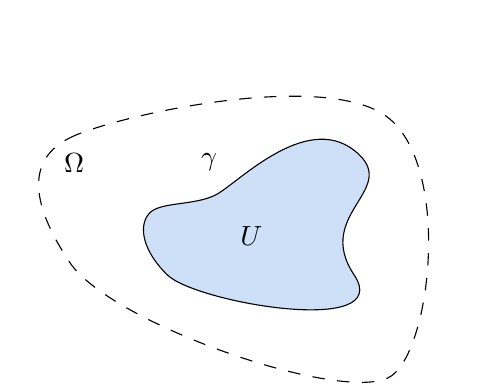
\begin{tikzpicture}[x=0.75pt,y=0.75pt,yscale=-1,xscale=1]
        %uncomment if require: \path (0,300); %set diagram left start at 0, and has height of 300
        
        %Shape: Polygon Curved [id:ds9387894112968782] 
        \draw  [fill={rgb, 255:red, 74; green, 144; blue, 226 }  ,fill opacity=0.28 ] (163.26,91.51) .. controls (173.26,86.51) and (206.26,51.51) .. (230,70) .. controls (253.74,88.49) and (210,100) .. (230,130) .. controls (250,160) and (153.74,143.49) .. (140,130) .. controls (126.26,116.51) and (126.44,104.14) .. (132.26,99.51) .. controls (138.07,94.89) and (153.26,96.51) .. (163.26,91.51) -- cycle ;
        %Shape: Polygon Curved [id:ds6099513547861319] 
        \draw  [dash pattern={on 4.5pt off 4.5pt}] (93,64) .. controls (113,54) and (207.26,32.51) .. (242.26,51.51) .. controls (277.26,70.51) and (268.26,163.51) .. (248.26,178.51) .. controls (228.26,193.51) and (113,154) .. (93,124) .. controls (73,94) and (73,74) .. (93,64) -- cycle ;
        
        % Text Node
        \draw (89,70.4) node [anchor=north west][inner sep=0.75pt]    {${\Omega}$};
        % Text Node
        \draw (174,105.4) node [anchor=north west][inner sep=0.75pt]    {$U$};
        % Text Node
        \draw (155,70.4) node [anchor=north west][inner sep=0.75pt]    {$\gamma $};
        
        
        \end{tikzpicture}
        \]
\end{theorem}
\begin{proof}[``Proof'']
    Let $U$ be the union of $\gamma$ and its interior. Let $f=u+iv$ as usual, write $\d z = \d x + i\d y$:\begin{align*}
        \int_{\gamma}f(z)\d z &= \int_\gamma (u+iv)(\d x + i\d y)\\
        &= \int_\gamma u\d x-v\d y + i\int_{\gamma}v\d x +u\d y\\
        &= \int\int_{U}(-v_x-u_y)\d x\d y+i\int\int_{U}(u_x-v_y)\d x\d y &&\text{by Green's thm}\\
        &= 0 &&\text{by Cauchy-Riemann}
    \end{align*}
\end{proof}
However, this `proof' heavily relies on the fact that $u,v$ are $C^1$ and that the partial derivatives are continuous. This assumes $f'$ is continuous, but we aren't sure about that yet!

\subsubsection{Take 2: deformation version}
\begin{theorem}[Cauchy's]\label[theorem]{cauchys-take2-deform}
    Let $\gamma_1,\gamma_2$ be piecewise $C^1$ curves in a region $\Omega$ with the same start and end points. If $\gamma_1$ can be continuously deformed to $\gamma_2$ without ever passing outside of $\Omega$, then \[\int_{\gamma_1}f(z)\d z=\int_{\gamma_2}f(z)\d z\]
\end{theorem}
By the \textit{previous} statement of Cauchy's theorem (in \cref{cauchys-take1}), we observe that $\int_{\gamma_1-\gamma_2}f(z)\d z=0$, so this one falls out.

\noneg The $\gamma_1,\gamma_2$ in the picture below cannot be continuously deformed into each other!
\[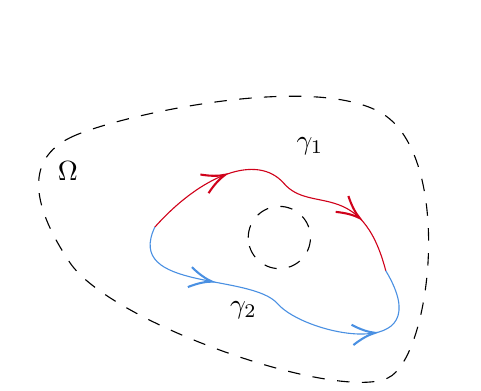
\begin{tikzpicture}[x=0.75pt,y=0.75pt,yscale=-1,xscale=1]
    %uncomment if require: \path (0,300); %set diagram left start at 0, and has height of 300
    
    %Shape: Polygon Curved [id:ds6460613846150254] 
    \draw  [dash pattern={on 4.5pt off 4.5pt}] (116,80) .. controls (136,70) and (230.26,48.51) .. (265.26,67.51) .. controls (300.26,86.51) and (291.26,179.51) .. (271.26,194.51) .. controls (251.26,209.51) and (136,170) .. (116,140) .. controls (96,110) and (96,90) .. (116,80) -- cycle ;
    %Curve Lines [id:da29780021147999514] 
    \draw [color={rgb, 255:red, 208; green, 2; blue, 27 }  ,draw opacity=1 ]   (157,123) .. controls (179.26,98.01) and (206.26,87.01) .. (219.26,102.01) .. controls (232.26,117.01) and (256.51,99.03) .. (268.26,144.01) ;
    \draw [shift={(190.93,97.76)}, rotate = 156.33] [color={rgb, 255:red, 208; green, 2; blue, 27 }  ,draw opacity=1 ][line width=0.75]    (10.93,-4.9) .. controls (6.95,-2.3) and (3.31,-0.67) .. (0,0) .. controls (3.31,0.67) and (6.95,2.3) .. (10.93,4.9)   ;
    \draw [shift={(255.72,118.67)}, rotate = 218.7] [color={rgb, 255:red, 208; green, 2; blue, 27 }  ,draw opacity=1 ][line width=0.75]    (10.93,-4.9) .. controls (6.95,-2.3) and (3.31,-0.67) .. (0,0) .. controls (3.31,0.67) and (6.95,2.3) .. (10.93,4.9)   ;
    %Curve Lines [id:da7249434898522338] 
    \draw [color={rgb, 255:red, 74; green, 144; blue, 226 }  ,draw opacity=1 ]   (157,123) .. controls (142.26,154.01) and (203.26,145.01) .. (216.26,160.01) .. controls (229.26,175.01) and (295.26,189.01) .. (268.26,144.01) ;
    \draw [shift={(184.59,149.25)}, rotate = 191.44] [color={rgb, 255:red, 74; green, 144; blue, 226 }  ,draw opacity=1 ][line width=0.75]    (10.93,-4.9) .. controls (6.95,-2.3) and (3.31,-0.67) .. (0,0) .. controls (3.31,0.67) and (6.95,2.3) .. (10.93,4.9)   ;
    \draw [shift={(263.11,173.95)}, rotate = 174.82] [color={rgb, 255:red, 74; green, 144; blue, 226 }  ,draw opacity=1 ][line width=0.75]    (10.93,-4.9) .. controls (6.95,-2.3) and (3.31,-0.67) .. (0,0) .. controls (3.31,0.67) and (6.95,2.3) .. (10.93,4.9)   ;
    %Shape: Circle [id:dp10939024496763072] 
    \draw  [dash pattern={on 4.5pt off 4.5pt}] (202,128.01) .. controls (202,119.73) and (208.71,113.01) .. (216.99,113.01) .. controls (225.27,113.01) and (231.99,119.73) .. (231.99,128.01) .. controls (231.99,136.29) and (225.27,143) .. (216.99,143) .. controls (208.71,143) and (202,136.29) .. (202,128.01) -- cycle ;
    
    % Text Node
    \draw (109,90.4) node [anchor=north west][inner sep=0.75pt]    {$\Omega $};
    % Text Node
    \draw (224,78.4) node [anchor=north west][inner sep=0.75pt]    {$\gamma _{1}$};
    % Text Node
    \draw (192,157.4) node [anchor=north west][inner sep=0.75pt]    {$\gamma _{2}$};
    
    
    \end{tikzpicture}
    \]

\subsection{Fresnel integrals}
Consider:
\[\int_{0}^{\infty}\sin (t^2)\d t \qquad \text{and} \qquad \int_{0}^{\infty}\cos (t^2)\d t\]
aka.
\[\lim_{R\to \infty}\int_{0}^{R}\sin (t^2)\d t \qquad \text{and} \qquad \lim_{R\to \infty}\int_{0}^{R}\cos (t^2)\d t\]
It's not obvious that these integrals converge!

Solution: PIZZA!
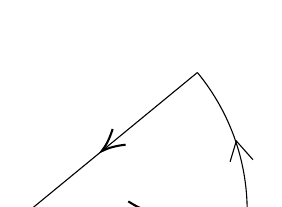
\begin{tikzpicture}[x=0.75pt,y=0.75pt,yscale=-1,xscale=1]
    %uncomment if require: \path (0,300); %set diagram left start at 0, and has height of 300
    
    %Straight Lines [id:da23065699869402656] 
    \draw    (100,126) -- (206.26,126) ;
    \draw [shift={(159.13,126)}, rotate = 180] [color={rgb, 255:red, 0; green, 0; blue, 0 }  ][line width=0.75]    (10.93,-4.9) .. controls (6.95,-2.3) and (3.31,-0.67) .. (0,0) .. controls (3.31,0.67) and (6.95,2.3) .. (10.93,4.9)   ;
    %Shape: Arc [id:dp010225998094383515] 
    \draw  [draw opacity=0] (205.5,126.02) .. controls (205.5,126.01) and (205.5,126.01) .. (205.5,126) .. controls (205.5,100.56) and (196.5,77.23) .. (181.5,59.01) -- (100,126) -- cycle ; \draw   (205.5,126.02) .. controls (205.5,126.01) and (205.5,126.01) .. (205.5,126) .. controls (205.5,100.56) and (196.5,77.23) .. (181.5,59.01) ;  
    %Straight Lines [id:da5834097312816091] 
    \draw    (100,126) -- (181.5,59.01) ;
    \draw [shift={(135.34,96.95)}, rotate = 320.58] [color={rgb, 255:red, 0; green, 0; blue, 0 }  ][line width=0.75]    (10.93,-4.9) .. controls (6.95,-2.3) and (3.31,-0.67) .. (0,0) .. controls (3.31,0.67) and (6.95,2.3) .. (10.93,4.9)   ;
    %Straight Lines [id:da6100230617755076] 
    \draw    (197.26,102.01) -- (200.26,92.01) -- (208.26,101.01) ;
    
    
    
    
    \end{tikzpicture}
Let $\gamma$ be the `sum' of all 3 curves as shown. Let $R\to \infty$. Then, by Cauchy's theorem, \(\int_\gamma e^{iz^2}\d z =0\).    

\ontangent{

\rmk We don't know how to write out the antiderivative of $f(z)=e^{iz^2}$ but we can use series!
\begin{align*}
    f(z) &= e^{iz^2}\\
    &= \sum_{n=0}^{\infty}\frac{(iz^2)^n}{n!}\\
    &= \sum_{n=0}^{\infty}\frac{i^nz^{2n}}{n!}
\end{align*}
And so \[F(z)=\sum_{n=0}^{\infty}\frac{i^nz^{2n+1}}{(2n+1)n!}\]

}

Now we return to the integral. Strategy: \[0= \int_\gamma e^{iz^2}\d  = \underset{I_1(R)}{\underbrace{\int_{\gamma_1} e^{iz^2}\d z}} + \underset{I_2(R)}{\underbrace{\int_{\gamma_2} e^{iz^2}\d z}} + \underset{I_3(R)}{\underbrace{\int_{\gamma_3} e^{iz^2}\d z}}\]

\[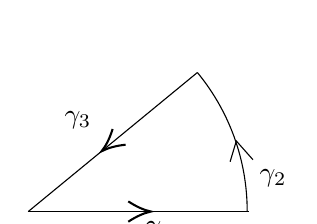
\begin{tikzpicture}[x=0.75pt,y=0.75pt,yscale=-1,xscale=1]
    %uncomment if require: \path (0,300); %set diagram left start at 0, and has height of 300
    
    %Straight Lines [id:da23065699869402656] 
    \draw    (100,126) -- (206.26,126) ;
    \draw [shift={(159.13,126)}, rotate = 180] [color={rgb, 255:red, 0; green, 0; blue, 0 }  ][line width=0.75]    (10.93,-4.9) .. controls (6.95,-2.3) and (3.31,-0.67) .. (0,0) .. controls (3.31,0.67) and (6.95,2.3) .. (10.93,4.9)   ;
    %Shape: Arc [id:dp010225998094383515] 
    \draw  [draw opacity=0] (205.5,126.02) .. controls (205.5,126.01) and (205.5,126.01) .. (205.5,126) .. controls (205.5,100.56) and (196.5,77.23) .. (181.5,59.01) -- (100,126) -- cycle ; \draw   (205.5,126.02) .. controls (205.5,126.01) and (205.5,126.01) .. (205.5,126) .. controls (205.5,100.56) and (196.5,77.23) .. (181.5,59.01) ;  
    %Straight Lines [id:da5834097312816091] 
    \draw    (100,126) -- (181.5,59.01) ;
    \draw [shift={(135.34,96.95)}, rotate = 320.58] [color={rgb, 255:red, 0; green, 0; blue, 0 }  ][line width=0.75]    (10.93,-4.9) .. controls (6.95,-2.3) and (3.31,-0.67) .. (0,0) .. controls (3.31,0.67) and (6.95,2.3) .. (10.93,4.9)   ;
    %Straight Lines [id:da6100230617755076] 
    \draw    (197.26,102.01) -- (200.26,92.01) -- (208.26,101.01) ;
    
    % Text Node
    \draw (155.13,129.4) node [anchor=north west][inner sep=0.75pt]    {$\gamma _{1}$};
    % Text Node
    \draw (210.26,104.41) node [anchor=north west][inner sep=0.75pt]    {$\gamma _{2}$};
    % Text Node
    \draw (116.26,76.41) node [anchor=north west][inner sep=0.75pt]    {$\gamma _{3}$};
    
    
    \end{tikzpicture}
    \]

Evaluate $I_1(R)$: We observe that $z$ is real for this one. Parameterize $z=t$ where $t$ is a real variable.
\begin{align*}
    I_1(R) &= \int_{\gamma_1} e^{it^2}\d t\\
    &= \int_{0}^{R}\cos (t^2)\d t + i\cdot \int_{0}^{R}\sin (t^2)\d t\\
\end{align*}
Hence, $\lim_{R\to \infty}I_1(R)= \int_{0}^{\infty}\cos (t^2)\d t + i\cdot \int_{0}^{\infty}\sin (t^2)\d t$.

Evaluate $I_2(R)$:

Parameterize $\gamma_2$ as $z=Re^{i\theta}$ where $\theta\in[0,\frac{\pi}{4}]$. Hence, $\d z = iRe^{i\theta}\d \theta$. Then:
\begin{align*}
    |I_2(R)| &= \left|\int_{\gamma_2} e^{i\theta^2}\d \theta\right|\\
    &= \left|\int_{0}^{\frac{\pi}{4}}e^{i(R e^{i\theta})^2}iRe^{i\theta}\d \theta\right|\\
    &= \left|R\int_{0}^{\frac{\pi}{4}}e^{iR^2e^{i2\theta}}e^{i\theta}\d \theta\right|\\
    &\leq R\int_{0}^{\frac{\pi}{4}}\left|e^{iR^2e^{i2\theta}}\right|\d \theta &&\text{by tri. ineq.}\\
    &\leq R\int_{0}^{\frac{\pi}{4}}e^{-R^2\sin2\theta}\d \theta&&\text{since when }x,y\in \R,\; \left|e^{x+iy}\right|=e^{x}\\
    &\leq  R\int_{0}^{\frac{\pi}{4}} e^{-R^2\frac{4\theta}{\pi}}\d \theta &&\text{since when }x\in [0,\frac{\pi}{2}],\; \frac{2}{\pi}x\leq \sin x\\
    &= \frac{-R\pi}{R^2 4}e^{-R\frac{4\theta}{\pi}}\bigg |_{\theta=0}^{\theta=\frac{\pi}{4}}\\
    &\to 0 \text{ as }R\to \infty
\end{align*}
Thus, $\lim_{R\to \infty}I_2(R)=0$. :)

Evaluate $I_3(R)$:
\begin{align*}
    I_3(R) &=\int_{\gamma_3} e^{iz^2}\d z\\
    &= \int_{R}^{0}e^{i(e^{i\frac{\pi}{4}}t)^2}e^{i\frac{\pi}{4}}\d t\\
    &= -e^{i\frac{\pi}{4}} \int_{0}^{R}e^{-t^2}\d t\\
    \lim_{R\to \infty} I_3(R) &= -(\frac{\sqrt{2}}{2}+i\frac{\sqrt{2}}{2})\int_{0}^{\infty}e^{-t^2}\d t &&\text{by Gaussian integral, }\int_{0}^{\infty}e^{-t^2}\d t = \frac{\sqrt{\pi}}{2}\\
    &= -\sqrt{\frac{\pi}{8}}-i\sqrt{\frac{\pi}{8}}
\end{align*}

Therefore, we see $I_1(R)+I_2(R)+I_3(R)=0$ where $\lim_{R\to \infty}I_1(R)= \int_{0}^{\infty}\cos (t^2)\d t + i\cdot \int_{0}^{\infty}\sin (t^2)\d t$, $I_2(R)\to 0$ and $I_3(R)= -\sqrt{\frac{\pi}{8}}-i\sqrt{\frac{\pi}{8}}$. Hence, we would be able to conclude that \[\int_{0}^{\infty}\sin (t^2)\d t = \sqrt{\frac{\pi}{8}} \qquad \text{and} \qquad \int_{0}^{\infty}\cos (t^2)\d t = \sqrt{\frac{\pi}{8}}\]

\end{document} 
